\chapter{Tổng quan nghiên cứu}
\label{chap:1tqnc}

\section{Giới thiệu robot tự hành}

% - Thế nào là robot tự hành thông minh
% - ứng dụng của robot tự hành thông

%%% Tài liệu tham khảo:
% http://ais.informatik.uni-freiburg.de/teaching/ss18/robotics/ Bài Introduction
%

Người ta coi cánh tay robot là robot truyền thống, bởi vậy khi nói đến thuật ngữ robot người ta thường nghĩ ngay đến cánh tay robot công nghiệp. \figurename{ \ref{fig:RBCongNghiep}} là hình ảnh các cánh tay robot đang làm việc trong dây chuyền sản xuất ô tô. Chúng ta không thấy bóng dáng con người ở trong bức hình này, bởi vì robot công nghiệp truyền thống phải làm việc trong không gian cách ly với con người, có hàng rào bảo vệ vì các lý do an toàn, con người không thể làm việc cùng không gian với robot.

\begin{figure}[hpt]
  \centering
  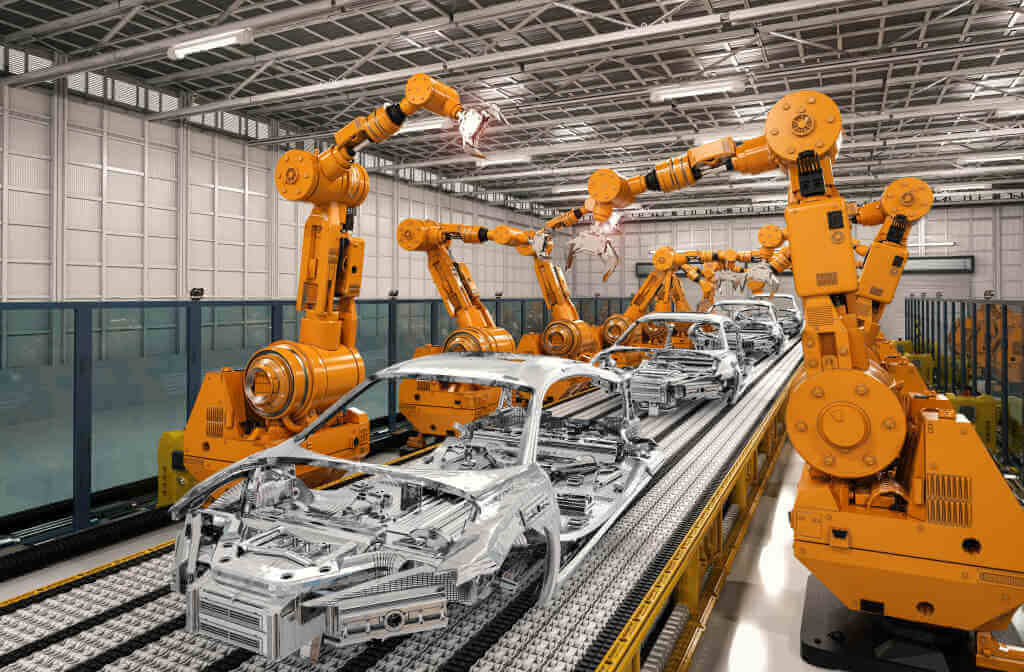
\includegraphics[width=10cm]{figures/IndustrialRobot.jpg}
  \caption[Robot công nghiệp]{Robot công nghiệp [Nguồn: Internet]}
  \label{fig:RBCongNghiep}
\end{figure}

Bên cạnh đó, robot di động (mobile robot) truyền thống thực hiện các nhiệm vụ di chuyển trên quỹ đạo xác định trước. Robot di động cũng hoạt động dựa trên các khối chương trình được lập trình sẵn. Các phương pháp điều khiển như điều khiển bằng tay thông qua bảng điều khiển, qua sóng RF, wifi... hay di chuyển bám đường chỉ dẫn gắn ở dưới sàn, đọc mã QR, bar. Các dạng robot này bị hạn chế về không gian hoạt động. Việc thiết lập, cấu hình nhà máy, không gian làm việc cho robot hoạt động rất tốn kém về chi phí và thời gian khiến chúng kém linh hoạt, khó có thể đáp ứng được các nhu cầu sản xuất thay đổi chóng mặt như hiện nay.

\begin{figure}
	\centering
    \subfloat[][]{
            \label{fig:rbMoi-a}
            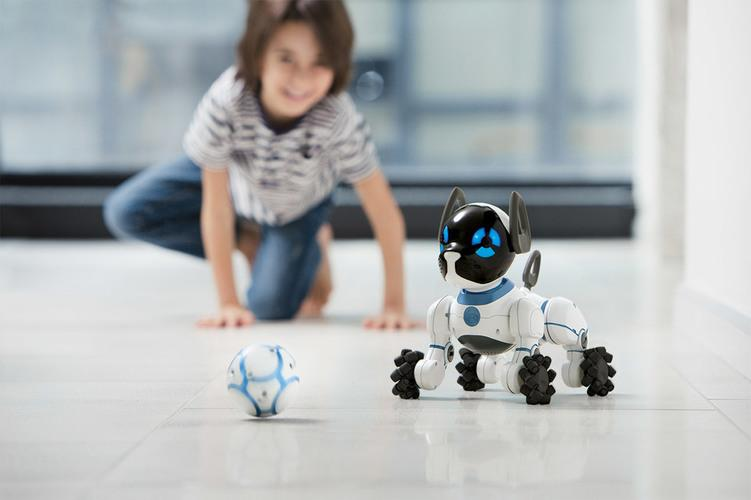
\includegraphics[height=5cm]{figures/c1_entertainmentRobot.jpg}}
            % \caption{Robot giải trí [\url{wowwee.com/chip}]}
          \subfloat[][]{
            \label{fig:rbMoi-b}
            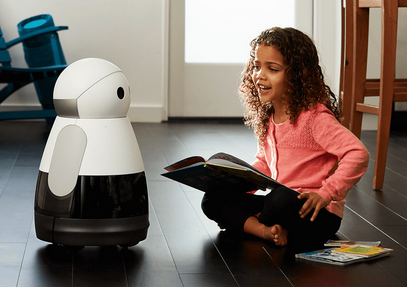
\includegraphics[height=5cm]{figures/c1_personalServiceRobot.png}}
        \hspace{8pt}
        \subfloat[][]{
          \label{fig:rbMoi-c}
          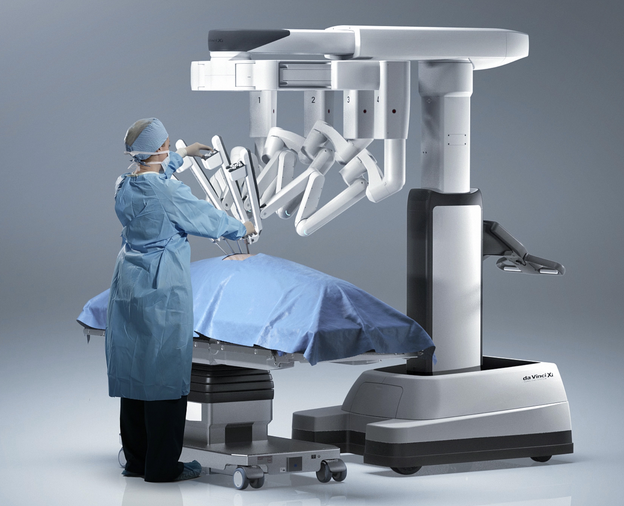
\includegraphics[height=4.6cm]{figures/c1_medicalRobot.png}}
        \subfloat[][]{
          \label{fig:rbMoi-d}
          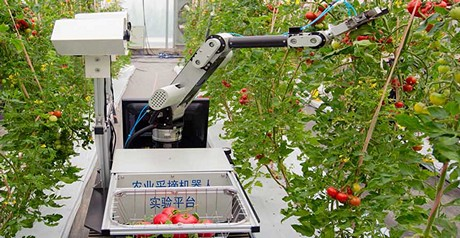
\includegraphics[height=4.6cm]{figures/c1_harvestingRobot.jpg}}
	\hspace{8pt}
	\caption[Một số loại robot mới]{Một số loại robot mới [Nguồn: Internet]}
	\label{fig:rbMoi}
\end{figure}

Ngày nay, robot có xu hướng trở nên thông minh hơn và xuất hiện nhiều loại robot có ứng dụng ngoài phạm vi nhà máy như:
robot giải trí (\figurename{ \ref{fig:rbMoi-a}}), robot dịch vụ cá nhân (\figurename{ \ref{fig:rbMoi-b}}) như máy tính cá nhân, robot trong y tế (\figurename{ \ref{fig:rbMoi-c}}); các loại robot tự động trong nông nghiệp như robot hái quả (\figurename{ \ref{fig:rbMoi-d}}), robot phun thuốc trong nông nghiệp, robot thông minh tác hợp trong công nghiệp; robot đi tới các môi trường mà con người không tới được như trong lòng đất dưới nước, trên không, trong vũ trụ. Ngoài ra, trong bối cảnh Thế giới và Việt Nam đang có những bước tiến mạnh mẽ trong cuộc cách mạng công nghiệp lần thứ tư, với xu hướng robot ngày một thông minh hơn, ứng dụng của robot tự hành ngày cảng lớn \cite{Ha2018}.

% robot giải trí (\figurename{ \ref{fig:rbMoi-a}} \footnote{\url{wowwee.com/chip}}),
% robot dịch vụ cá nhân (\figurename{ \ref{fig:rbMoi-b}} \footnote{\url{www.noithatmagazine.vn/amazon-dang-phat-trien-robot-quan-gia-648592.html}}) (như máy tính cá nhân), robot trong y tế (\figurename{ \ref{fig:rbMoi-c}} \footnote{\url{www.overlakehospital.org/robot}}); các loại robot tự động trong nông nghiệp như robot hái quả (\figurename{ \ref{fig:rbMoi-d}} \footnote{\href{www.freshplaza.com/article/175737/Mechanical-harvesting-robot-received-attention-at-Macfrut/}{www.freshplaza.com}}), phun thuốc trong nông nghiệp, robot thông minh tác hợp trong công nghiệp; robot đi tới các môi trường mà con người không tới được như trong lòng đất dưới nước, trên không, trong vũ trụ...

\begin{figure}[htp]
  \centering
  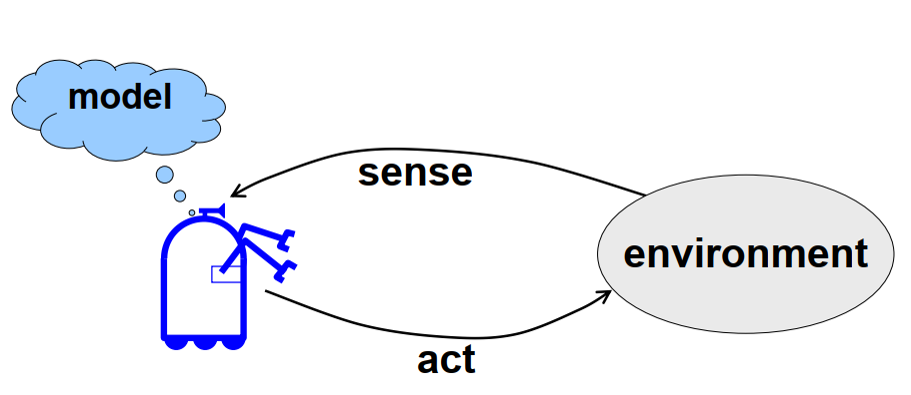
\includegraphics[width=12cm]{figures/c1_AutonomousRBModel.png}
  \caption{Mô hình hệ thống robot tự hành \cite{Burgard2018}}
  \label{fig:MohinhRB}
\end{figure}

Robot tự hành thông minh là một loại robot di động. Robot có thể cảm nhận môi trường thông qua hệ thống cảm biến, sử dụng các mô hình học máy để mô hình hóa môi trường. Từ đó, robot có thể thực hiện các hành động phản ứng lại với môi trường như di chuyển và một số hành động khác theo yêu cầu (\figurename{ \ref{fig:MohinhRB}}).

% Có nên thêm phần giới thiệu các robot dựa trên robot tự hành:

\section{Ứng dụng của robot tự hành thông minh}
\label{sec:ungdung}
%==============================================

Với sự thông minh và linh hoạt, robot tự hành thông minh có rất nhiều ứng dụng. Về cơ bản, đây là nền tảng để di chuyển cho hầu hết các loại robot di động thông minh ngày nay. Sản phẩm ứng dụng của robot tự hành thông minh khá đa dạng như:

\begin{itemize}
  \item Ứng dụng trong nhà như robot hút bụi thông minh, robot dịch vụ thông minh, robot vận chuyển trong các nhà máy, kho hàng
  \item Ứng dụng ngoài trời như robot cắt cỏ, robot chăm sóc cây trồng
  \item Robot làm việc tại các không gian mà con người không tới được như robot thám hiểm dưới nước, trong lòng đất, trên không trung, trên vũ trụ
  \item Và đặc biệt phát triển nhanh trong những năm gần đây là xe tự lái, robot giao hàng tự động.
\end{itemize}

\section{Các bài toán trên robot tự hành thông minh}
% - Nêu qua concept về điều khiển robot, tạo bản đồ, định vị, path planning, điều hướng, tránh vật cản
%=================================================

Di chuyển là một khả năng bẩm sinh của động vật nói chung và con người nói riêng, chúng ta di chuyển rất dễ dàng. Tuy nhiên, đối với robot linh hoạt trong môi trường động không hề đơn giản, robot phải xử lý nhiều bài toán phức tạp.
Dưới đây là một số bài toán chính trong robot tự hành thông minh (\cite{Wise}):

\textbf{Xử lý tín hiệu cảm biến:} Robot tự hành thông minh cần một số loại cảm biến để có thể hiểu được môi trường, định vị và di chuyển tránh vật cản.

Có rất nhiều loại cảm biến cho robt để cảm nhận được đa dạng thông tin của môi trường. Có thể chia làm các nhóm như sau:
\begin{itemize}
\item Cảm biến khoảng cách một chiều: Cảm biến khoảng cách hồng ngoại, siêu âm
\item Cảm biến khoảng cách hai chiều: Lidar
\item Cảm biến hình ảnh 3 chiều như Intel realsense, Microsoft Kinect, Asus Xction...
\item Ước tính trạng thái robot: GPS, IMU
\item Cảm biến lực, momen, cảm biến chạm...
\item Cảm biến âm thanh, giọng nói như microphone, microphone array
\item Các loại camera 2D
\end{itemize}

\textbf{Odometry}: Là bài toán sử dụng thông tin nhận được từ các cảm biến của robot để ước tính sự thay đổi vị trí của robot qua thời gian. Odometry được sử dụng trong hầu hết các robot tự hành.

\textbf{Định vị}: Bài toán định vị giúp trả lời câu hỏi robot đang ở đâu, từ đó có cơ sở để thực hiện các tác vụ khác như tạo bản đồ, xác định hướng di chuyển.

\textbf{Xây dựng bản đồ}: Dự trên dữ liệu từ các loại cảm biến, từ odometry và định vị robot, robot sử dụng các thuật toán để xây dựng bản đồ của môi trường.

\textbf{Kế hoạch di chuyển và điều hướng robot}: Sau khi có bản đồ, để thực hiện nhiệm vụ đi từ vị trí hiện tại tới một vị trí đích xác định. Robot sẽ tính toán, lập kế hoạch di chuyển và điều khiển robot di chuyển tới đích.

\textbf{Tránh vật cản}: Trong quá trình di chuyển, robot phát hiện được các vật cản (bao gồm cả tĩnh và động) và tránh vật cản, sau đó thiết lập lại quỹ đạo di chuyển tới đích.

Vấn đề xuyên suốt trong các bài toán của robot tự hành thông minh đó là các dữ liệu đều không chắc chắn, các bài toán trên đều dựa vào các mô hình xác suất để mô hình hóa được trình bày trong tài liệu \cite{thrun2005probabilistic}.

% Thêm một đoạn dẫn liên kết vào đây

\section{Các nghiên cứu tránh vật cản trong robot tự hành thông minh}
\label{sec:tranhVatCan_ref}
% Review các bài báo về tránh vật cản trong robot tự hành
% Chỉ ra các ưu, nhược điểm của các phương pháp như được nêu trong các bài báo trên
%================================================================

Khả năng phát hiện và tránh vật cản theo thời gian thực là rất quan trọng trong robot tự hành. Do đó có rất nhiều nghiên cứu về giải pháp cho vấn đề này. Có nhiều loại cảm biến, nhiều giải thuật được sử dụng.
Có các loại cảm biến sử dụng như cảm biến khoảng cách hồng ngoại, siêu âm với ứng dụng trên các thiết bị nhúng cấu hình thấp \cite{dongyue2013, Susnea2009}. Các phương pháp sử dụng cảm biến laser radar được trình bày trong \cite{Gao2019, Wu2015, Peng2015,Baras2019}.

Một số thuật toán phổ biến được dùng để phát hiện và tránh vật cản như Virtual Force Field (VFF - Trường lực ảo) \cite{Borenstein1989}, Vector Field Histogram (VFH - Biểu đồ trường lực) \cite{Borenstein1991}, Dynamic Window Approach (DWA - Cửa sổ tiếp cận động) \cite{Fox1997}\ldots

Sau đây, các thuật toán sẽ được giới thiệu chi tiết.

\subsection{Thuật toán Virtual Force Field (VFF)}
%------------------------------------------------

Được áp dụng cho điều khiển tránh vật cản trình bày trong \cite{Borenstein1988,Borenstein1989}. Ý tưởng của giải thuật này là tạo một ô lưới quanh robot. Khi có dữ liệu có vật cản từ cảm biến, ô tương ứng sẽ được đặt là bị chiếm dụng bởi vật cản với một tỉ số chiếm dụng (thể hiện cho sự không chắc chắn), nhiệm vụ của thuật toán là tính toán một lực để đưa robot xa khỏi ô bị chiếm dụng đó theo công thức \ref{equa:Fij}


\begin{equation}
  F(i,j) = \frac{{F}_{cr}C(i,j)}{{d}^{2}(i,j)}\left [\frac{{x}_{t}-{x}_{0}}{d(i,j)}\dot{x} + \frac{{y}_{t}-{y}_{0}}{d(i,j)}\dot{y}
  \right ]
  \label{equa:Fij}
\end{equation}
Trong đó:

\begin{tabular}{ll}
  $F(i,j)$      & Lực ảo chống lại vật cản tại ô (i,j) \\
  ${F}_{cr}$    & Hằng số lực chống lại vật cản  \\
  $d(i,j)$      & Khoảng cách giữa ô (i,j) và robot \\
  ${C}_{i,j}$   & Độ chắc chắn tại ô (i,j)  \\
  ${x}_{0}, {y}_{0}$ & Tọa độ robot \\
  ${x}_{i}, {y}_{j}$ & Tọa độ của ô (i,j)
\end{tabular}

Lực ${F}_{r}$ đưa robot tránh khỏi các vật cản xuất hiện xung quanh robot là tổng của các lực đưa robot tránh các ô bị chiếm dụng

\begin{equation}
  {F}_{r} = \sum\limits_{i,j}{F(i,j)}
\end{equation}

Trong khi đó, lực ${F}_{t}$ kéo robot đi từ điểm hiện tại tới điểm đích như sau:

\begin{equation}
  {F}_{t} = {F}_{ct} \left [\frac{{x}_{t}-{x}_{0}}{d(t)}\dot{x} + \frac{{y}_{t}-{y}_{0}}{d(t)}\dot{y}
  \right ]
\end{equation}

Trong đó:

\begin{tabular} {ll}
  ${F}_{ct}$    & Hằng số lực kéo robot tới đích \\
  $d(t)$        & Khoảng cách giữa robot và điểm đích \\
  ${x}_{t}, {y}_{t}$ & Tọa độ của điểm đích
\end{tabular}

\begin{figure}[htp]
  \centering
  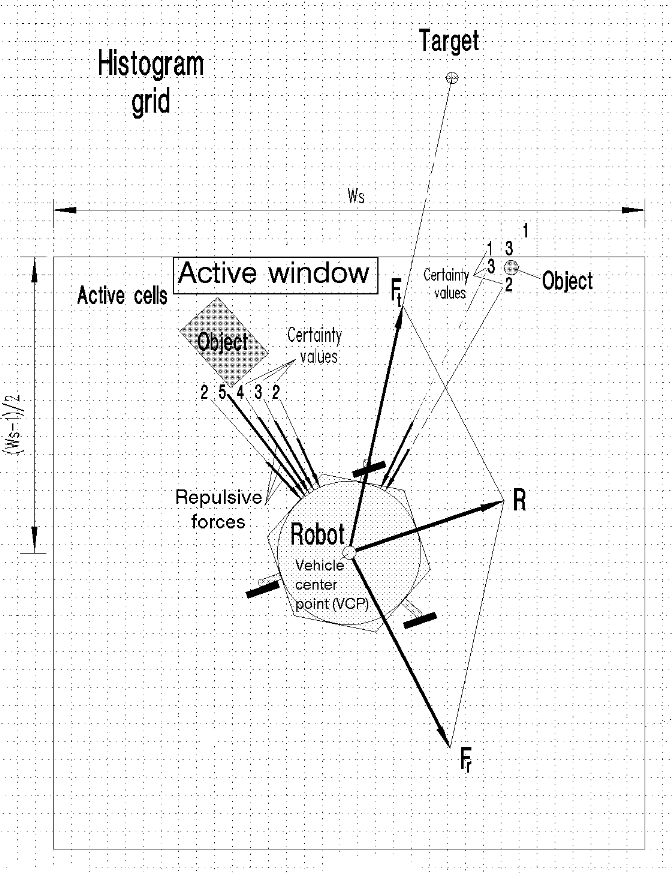
\includegraphics[width=1\linewidth]{figures/VFFconcept.png}
  \caption{Virtual Force Field \cite{Koren1991}}
  \label{fig:VFFconcept}
\end{figure}

Hợp lực của 2 loại lực này là lực chính kéo robot di chuyển (\figurename{ \ref{fig:VFFconcept}}).

\begin{equation}
  R = {F}_{t} + {F}_{r}
\end{equation}


Từ đó tính được hướng di chuyển của robot để điều khiển bánh xe di chuyển, đưa robot tới đích và tránh được vật cản. Theo \cite{Borenstein1988}, phương pháp này có một số ưu điểm như sau:
\begin{itemize}
  \item Phương pháp này không xác định được đường viền cạnh của vật cản, nhưng có thể xác định được cụm các vị trí có vật cản.
  \item Phương pháp này không yêu cầu robot phải dừng lại để thực hiện lấy dữ liệu và tính toán. Trong điều kiện lý tưởng, phương pháp này giúp robot có thể tránh được tất cả vật cản trong khi vẫn di chuyển với vận tốc tối đa.
  \item Việc cập nhật bản đồ lưới và điều hướng sử dụng bản đồ lưới là hai nhiệm vụ hoàn toàn không phụ thuộc vào nhau, nhưng có thể đồng bộ với nhau để tối ưu tính toán.
  \item Phương pháp này có thể dễ dàng tích hợp nhiều loại cảm biến để bổ sung thông tin vào bản đồ ô lưới.
\end{itemize}

Tuy nhiên theo \cite{Koren1991}, phương pháp này có một số điểm hạn chế như: có một số trường hợp mắc bẫy do cực tiểu địa phương, không thể di chuyển qua giữa các vật cản gần nhau, lưỡng lự khi có vật cản, lưỡng lự trong lối đi hẹp

Do đó, phương pháp Vector Field Histogram cải thiện các hạn chế của phương pháp Vector Force Field

\subsection{The Vector Field Histogram}
\label{sub:VFH}
%-------------------------------------

\begin{figure}[htbp]
  \centering
  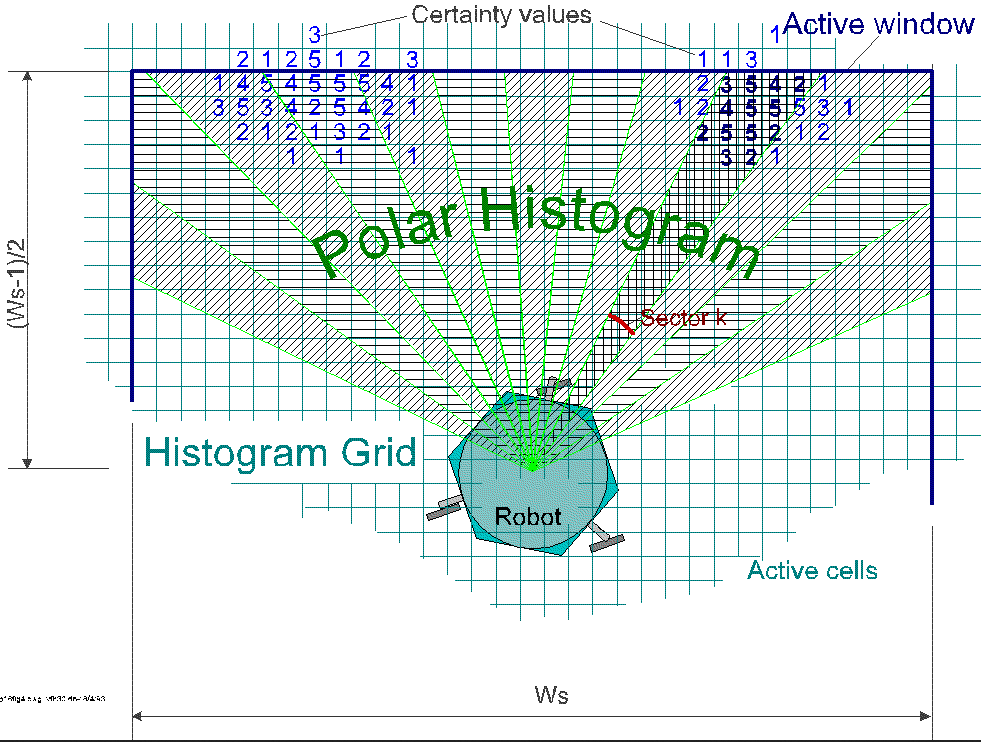
\includegraphics[width=0.6\linewidth]{figures/VFH-PolarHistogram.png}
  \caption{Biểu đồ cực trong VFH}
  \label{fig:PolarHistogram}
\end{figure}

Phương pháp VFH được trình bày chi tiết trong \cite{Borenstein1991}. Phương pháp này sử dụng một cấu trúc dữ liệu trung gian, được gọi là biểu đồ cực H (\textit{polar histogram}). H là một mảng 72 góc hình quạt (\figurename{ \ref{fig:PolarHistogram}}).

Phương pháp này sử dụng kĩ thuật hai giai đoạn giảm dữ liệu và ba mức thể hiện dữ liệu:

\begin{itemize}
  \item Mức biểu diễn dữ liệu cao nhất giữ mô tả chi tiết của môi trường robot, bản đồ lưới 2 chiều được cập nhật liên tục theo thời gian thực như trong phương pháp VFF.
  \item Mức ở giữa, một biểu đồ H một chiều được dựng quanh vị trí tức thời của robot. H bao gồm $n$ góc với độ rộng $\alpha$, phép chuyển đổi từ C sang H.
  \item Mức biểu diễn dữ liệu thấp nhất là đầu ra của thuật toán VFH: các giá trị tham chiếu cho động cơ và bánh xe điều khiển robot.
\end{itemize}

\begin{figure}[htbp]
  \centering
  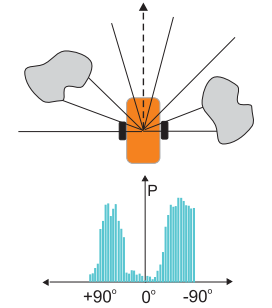
\includegraphics[width=0.6\textwidth]{figures/VFH.png}
  \caption{Vector Field Histogram \cite{Susnea2009}}
  \label{fig:VFH}
\end{figure}

Phương pháp này có thể phát hiện được lối đi đủ cho robot đi qua giữa các vật cản. Phương pháp VFF dễ bị ảnh hưởng bởi sai số của cảm biến, với phương pháp này, sử dụng làm mịn biểu đồ H đã giảm trọng số của các giá trị sai ngẫu nhiên của cảm biến, do đó phương pháp này mạnh hơn phương pháp VFF. Vẫn bị hiện tượng mắc bẫy khi vào các trường hợp đường cụt (dead-end) do sử dụng phương pháp cục bộ. Tốc độ di chuyển tối đa khi điều khiển robot bằng VFH bị giới hạn bởi tốc độ lấy mẫu của cảm biến.

Dựa trên phương pháp này, tác giả tài liệu \cite{Ulrich1998} đã đề xuất phương pháp được gọi là VFH+ thực hiện 4 giai đoạn giảm dữ liệu từ bản đồ lưới chiếm dụng hai chiều xuống thành dữ liệu điều khiển hướng di chuyển của robot. Sử dụng một số cải tiến để giúp robot có thể di chuyển tốt hơn.

\subsection{Phương pháp "Bong bóng phản ứng" tránh vật cản}
%---------------------------------------------------------

% \begin{wrapfigure}{r}{0.5\textwidth}
%   \centering
%   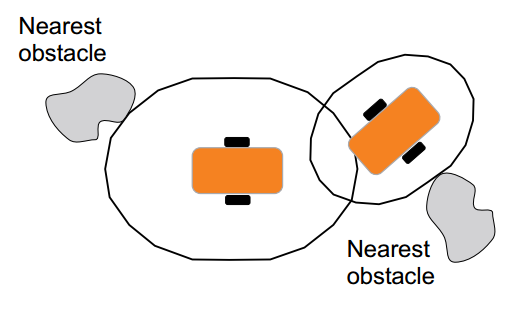
\includegraphics[width=0.5\textwidth]{figures/bubble-band.png}
%   \caption{Bong bóng phản ứng \cite{Susnea2009}}
%   \label{fig:bubble-band}
% \end{wrapfigure}

\begin{figure}[htbp]
  \centering
  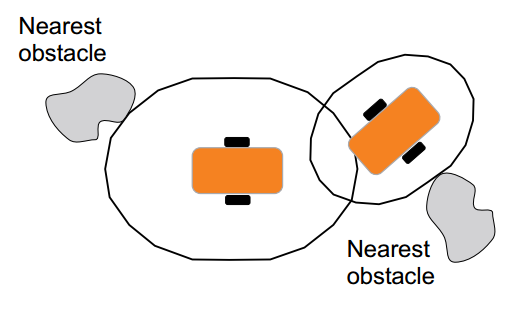
\includegraphics[width=0.6\linewidth]{figures/bubble-band.png}
  \caption{Bong bóng phản ứng \cite{Susnea2009}}
  \label{fig:bubble-band}
\end{figure}


Phương pháp này được đề xuất trong \cite{Quinlan1993}, phương pháp này định nghĩa một "bong bóng" bao quanh robot thể hiện không gian lớn nhất có thể di chuyển mà không gặp vật cản trong một khoảng thời gian. Hình dạng và kích thước của bong bóng được xác định đơn giản dựa trên hình dạng vật lý của đế robot và từ thông tin của cảm biến (như \figurename{ \ref{fig:bubble-band}}).

\begin{figure}[htbp]
	\centering
	\subfloat[]{
          \label{fig:bb-computeAngle}
          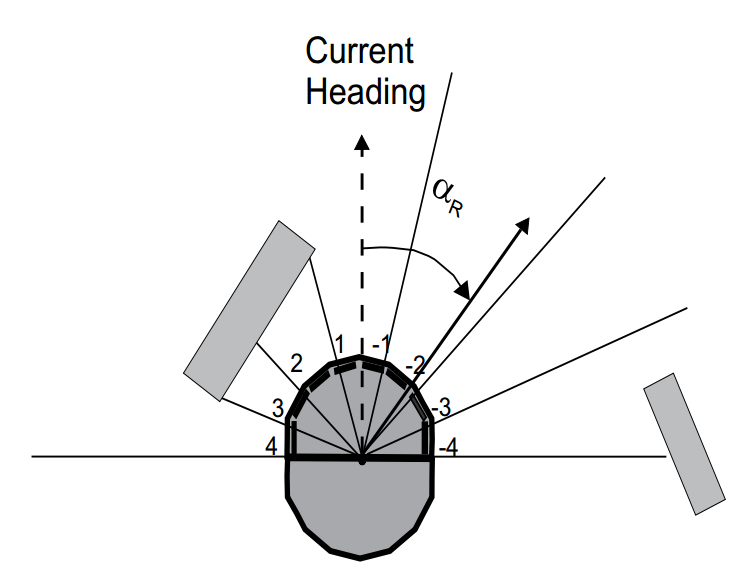
\includegraphics[width=0.45\textwidth]{figures/computeReboundAngle.png}}
  \subfloat[]{
          \label{fig:bb-reboudProcess}
          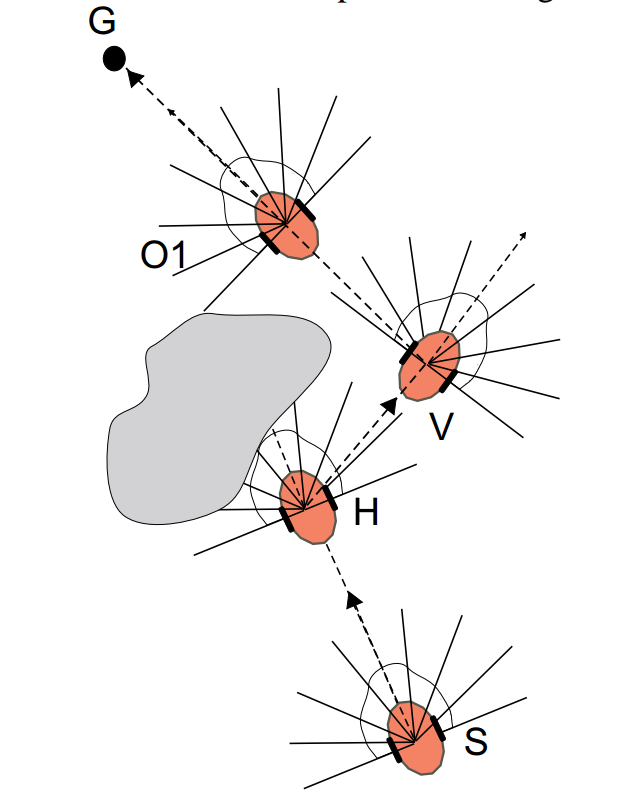
\includegraphics[width=0.4\textwidth]{figures/rebound.png}}
	\caption{Phương pháp bong bóng phản ứng động}
	\label{fig:bubbleRebound}
\end{figure}

Một phương pháp cải tiến được đề xuất trong \cite{Susnea2010}. Tác giả đã cải tiến hình dạng của bong bóng, không phải là hình dạng cố định như trong \cite{Quinlan1993} mà hình dạng và kích thước được điều chỉnh liên tục dựa vào tốc độ di chuyển của robot. Khi các cảm biến phát hiện vật cản nằm trong giới hạn của bong bóng phản ứng, một thuật toán được dùng để xác định hướng của vật cản so với hướng di chuyển của robot \figurename{ \ref{fig:bb-computeAngle}}. Một quá trình di chuyển của robot sử dụng phương pháp này được minh họa tại \figurename{ \ref{fig:bb-reboudProcess}}.

Cũng theo tác giả trong tài liệu \cite{Susnea2010}, phương pháp này có ưu điểm là có thể triển khai trên các thiết bị giá thành thấp, chi phí tính toán thấp nhưng có thể hoạt động theo thời gian thực. Tuy nhiên, nó cũng có một số điểm hạn chế như quá trình di chuyển chưa mượt, robot khó xử lý khi gặp nhiều vật cản đồng thời.

\subsection{Tránh vật cản cho thiết bị tự hành bằng LIDAR và hệ thống nhúng}
  Tài liệu \cite{Baras2019} tác giả trình bày một mô hình robot tự hành di chuyển và tránh vật cản sử dụng RPLidar A2 và máy tính nhúng Raspberry Pi 3. Tóm tắt hệ thống như sau:

  \begin{figure}[htbp]
    \centering
    \subfloat[]{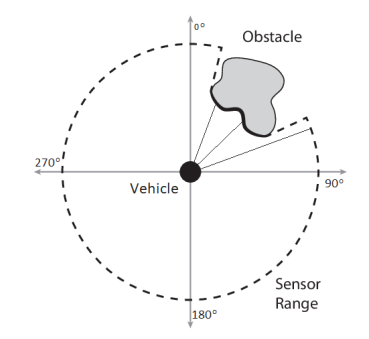
\includegraphics[width=0.45\linewidth]{figures/refer_lidar-apply-obstacle-detect.png}}
    \qquad
    \subfloat[]{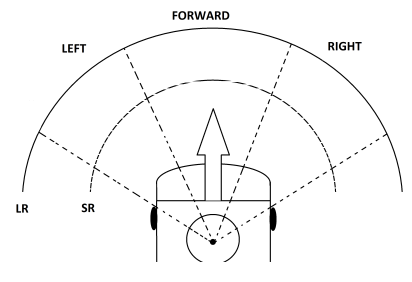
\includegraphics[width=0.45\linewidth]{figures/refer_lidar-apply.png}}
    \caption[Xác định vị trí vật cản]{Xác định vị trí vật cản. Hình a thể hiện laser quét phát hiện vật cản. Hình b thể hiện phân vùng vị trí vật cản}
    \label{fig:lidar-apply}
  \end{figure}

  \begin{itemize}
    \item \textbf{Hệ thống định vị trong nhà:} Trong tài liệu này tác giả sử dụng phương pháp định vị IPS (Indoor Positioning System - Hệ thống định vị trong nhà), sử dụng hạ tầng Wi-Fi sẵn có. Nhiều trạm phát Wi-Fi được đặt trong không gian. Dựa vào cường độ tín hiệu Wi-Fi có thể tính được khoảng cách tới trạm phát Wi-Fi đó. Cần ít nhất 3 trạm phát sóng Wi-Fi để xác định được vị trí của robot.
    \item \textbf{Phát hiện vật cản:} Module RPLidar A2 được sử dụng để phát hiện vật cản xung quanh robot. Dựa trên góc quét của Lidar, tác giả chia thành 4 vùng: Trước, Trái, Phải và Sau (Hình \ref{fig:lidar-apply})

    \item \textbf{Tránh vật cản:} Hệ thống IPS dẫn robot đi từ vị trí hiện tại tới đích, trong quá trình di chuyển đó module RPLidar liên tục quét để phát hiện vật cản. Nếu vùng phía trước, trái và phải không có vật cản, robot sẽ di chuyển theo đường ngắn nhất để tới đích. Nếu phía có xuất hiện vật cản tại hướng nào đó, robot sẽ xem xét các hướng còn lại và quyết định đi theo hướng nào.
  \end{itemize}



  Tài liệu này đề xuất phương pháp định vị, dẫn đường và tránh vật cản rất đơn giản, có thể hiệu quả nhưng vẫn còn nhiều hạn chế. Chưa có bản đồ để có thể xác định kế hoạch di chuyển tối ưu nhất. Phần tránh vật cản có thể khiển robot dễ rơi vào các trạng thái không thể di chuyển do xuất hiện nhiều vật cản mà không quyết định được để len lỏi giữa chúng.

\subsection*{Kết luận}
Trên đây là một số phương pháp tránh vật cản và điều hướng cho robot. Các phương pháp trên là các phương pháp sơ khai và tương đối đơn giản với các ưu điểm có thể triển khai trên các thiết bị nhúng, nhẹ, chi phí tính toán thấp nhưng vẫn đảm bảo hoạt động theo thời gian thực.

Tuy nhiên, các phương pháp trên có những hạn chế về định vị, dẫn đường và tránh vật cản:
\begin{itemize}
  \item Chưa có bản đồ của môi trường
  \item Hệ thống điều hướng chưa tốt
  \item Chỉ mới phát hiện và tránh vật cản trên một mặt phẳng bố trí cảm biến.
\end{itemize}

Trong luận văn này, tác giả sẽ ứng dụng nền tảng robot tự hành có sẵn. Với khả năng định vị, dẫn đường, tạo bản đồ trên nền tảng hệ điều hành robot ROS và giải thuật SLAM. Từ đó, tác giả đề xuất phương pháp tăng độ an toàn trong quá trình di chuyển bằng cách thêm một tầng cảm biến tránh vật cản cho robot, áp dụng thuật toán tránh vật cản và phối hợp nhiều tầng cảm biến điều khiển robot.

\section{Nội dung nghiên cứu}
% Chốt lại nội dung nghiên cứu gồm 2 nội dung:
% - Điều khiển robot ứng dụng SLAM trên nền tảng hệ điều hành ROS
% - Sử dụng Multi-sensor để tăng cường phát hiện và tránh vật cản cho robot
% - Trình bày vắn tắt nội dung của các chương.
%===========================================
Nội dung nghiên cứu chính của luận văn gồm ba phần như sau:

\begin{itemize}
  \item Nghiên cứu hệ thống định vị, di chuyển và tạo bản đồ dựa trên nền tảng hệ điều hành ROS và ứng dụng vào điều khiển robot tự hành Dashgo D1.
  \item Tăng cường phát hiện và tránh vật cản cho robot bằng đa tầng cảm biến. Đề xuất phương pháp lắp đặt cảm biến và giải thuật điều khiển, phân quyền điều khiển robot
  \item Thực hiện đánh giá hiệu quả của hệ thống.
\end{itemize}

Nội dung của luận văn như sau: Chương 1 khái quát tổng quan về robot tự hành, một số phương pháp điều khiển và tránh vật cản được sử dụng trong robot tự hành. Chương 2 tổng hợp một số cơ sở lý thuyết được sử dụng trong luận văn này, bao gồm bài toán về nhiễu và xác suất trong robot tự hành, hệ điều hành robot ROS, bài toán điều hướng robot, bài toán SLAM 2D. Chương 3 trình bày giải thuật và phương pháp triển khai để kiểm chứng hiệu quả của giải thuật tránh vật cản do tác giả đề xuất. Chương 4 là kết luận của tác giả về các vấn đề trong luận văn, từ đó đề xuất các hướng phát triển sau này.

%%===========================
\chapter{Cơ sở lý thuyết}
\label{chap:1cslt}
\section{Bài toán về nhiễu trong robot tự hành \cite{thrun2005probabilistic}}
\label{sec:2.1}

\subsection{Sự không chắc chắn trong robot}
Robotics là một ngành khoa học về nhận thức và thực thi thế giới vật lý thông qua các thiết bị điều khiển bởi máy tính. Một số ví dụ thành công của hệ thống robotics như robot di động khám phá hành tinh, robot công nghiệp trong dây chuyền sản xuất, xe tự lái, cánh tay robot hỗ trợ bác sĩ phẫu thuật. Các hệ thống robotics được đặt trong thế giới vật lý, quan sát thông tin môi trường thông qua các cảm biến, và thao tác thông qua các lực vật lý.
% Đặc biệt trong công nghệ robot tự hành, robot phải có khả năng đáp ứng rất lớn sự không chắc chắn tồn tại trong thế giới vật lý.

Trong khi ngành robotics vẫn còn trong thời kì trứng nước, ý thưởng các thiêt bị thực thi thông minh mang tới khả năng to lớn để thay đổi thế giới. Sẽ rất tuyệt vời nếu tất cả xe hơi đều có thể tự lái an toàn và tránh được hoàn toàn tai nạn giao thông. Sẽ rất tuyệt vời nếu robot có thể tự nó hoạt động để làm sạch chất phóng xạ trong thảm họa hạt nhân thay cho con người. Sẽ rất tuyệt vời nếu nhà của chúng ta có các thiết bị hỗ trợ thông minh để quản lý sửa chữa, duy tu các đồ vật trong nhà. Để làm được những việc này, robot phải có khả năng đáp ứng độ không chắc chắn rất lớn trong thế giới vật lý. Có rất nhiều yếu tố tạo nên sự không chắc chắn trong robot.

Trước hết, môi trường của robot vốn dĩ đã không ổn định. Trong các môi trường có cấu trúc tốt, được thiết kế theo tiêu chuẩn như trong dây chuyền lắp ráp thì mức độ không chắc chắn thấp, trong khi đó các môi trường khác như môi trường trong nhà của robot dịch vụ hay trên đường phố có mức độ không chắc chắn cao, có nhiều biến động. Với các robot hoạt động gần con người thì độ không chắc chắn rất cao.

Robot sử dụng hệ thống cảm biến để cảm nhận, quan sát môi trường xung quanh. Tuy nhiên, cảm biến có các giới hạn quan sát của nó. Phạm vi và độ phân giải của một cảm biến phụ thuộc vào giới hạn vật lý. Ví dụ, các camera không thể nhìn xuyên tường, độ phân giải của camera cũng có giới hạn. Cảm biến rất khó tránh khỏi nhiễu, và các phép đo nhiễu không thể đoán trước được. Do đó nó giới hạn thông tin có thể trích xuất được từ cảm biến. Hoặc cảm biến có thể bị hỏng và việc phát hiện lỗi từ cảm biến vô cùng khó khó khăn.

Robot được dẫn động bằng động cơ, ở một mức độ nhất định nó cũng không dự đoán được sai số. Độ không chắc chắn sinh ra do ảnh hưởng từ nhiễu điều khiển, mòn bánh răng và các lỗi cơ khí khác. Một vài cơ cấu chấp hành như cánh tay robot công nghiệp thường rất chính xác và độ tin cậy cao. Còn lại, như các robot di động giá thành thấp có thể rất dễ hỏng.

Nhiều nguyên nhân không chắc chắn có thể đến từ phần mềm của robot. Tất cả mô hình của thế giới vật lý đều gần đúng. Mô hình là trừu tượng hóa của thế giới thực, vì vậy, chúng ta chỉ có thể mô hình được một phần các quá trình vật lý cơ bản của robot và môi trường hoạt động của nó. Lỗi mô hình hóa dẫn đến sự không chắc chắn thường bị bỏ qua trong quá trình chế tạo robot, mặc dù thực tế là hầu hết các mô hình robot được sử dụng trong các hệ thống robot hiện đại khá thô sơ.

Sự không chắc chắn cũng có thể do các thuật toán gần đúng. Các hệ thống điều khiển robot có thể bị hạn chế lượng tính toán để đảm bảo robot có thể hoạt động theo thời gian thực. Đa số các thuật toán đều gần đúng, việc đảm bảo thời gian phản hồi có thể bị đánh đổi bởi độ chính xác.

Mức độ không chắc chắn phụ thuộc vào lĩnh vực ứng dụng. Trong một vài lĩnh vực robotics, như dây chuyền lắp ráp độ không chắc chắn có thể chỉ là các yếu tố nhỏ, bên ngoài. Tuy nhiên, trong robot tự hành, mức độ không chắc chắn là rất lớn, nó đến từ việc hoạt động trong môi trường động, từ sai số của các cảm biến, từ sai số trong mô hình hóa chính robot \dots

\subsection{Xác suất trong robotics} \label{subsec:probabilityinRobotics}

Xác suất trong robot có liên quan tới cách tiếp cận mới để giải quyết vấn đề trong quan sát và hành động của robot, đặc biệt là với robot tự hành. Ý tưởng chính trong bài toán xác suất trong robot là thể hiện sự không chắc chắn một cách rõ ràng bằng việc sử dụng lý thuyết tính toán xác suất. Nhưng thay vì dựa vào một "dự đoán tốt nhất" thay cho những gì có thể xảy ra, các thuật toán xác suất thể hiện thông tin bằng các phân bố xác suất qua toàn bộ không gian dự đoán. Như vậy, chúng có thể biểu diễn sự không chắc chắn và độ tin cậy trong toán học. Xác suất trong robot có thể chủ động lựa chọn để giảm sự không chắc chắn, do đó các thuật toán xác suất giảm độ phức tạp của sự không chắc chắn.

\begin{figure}[htbp]
  \centering
  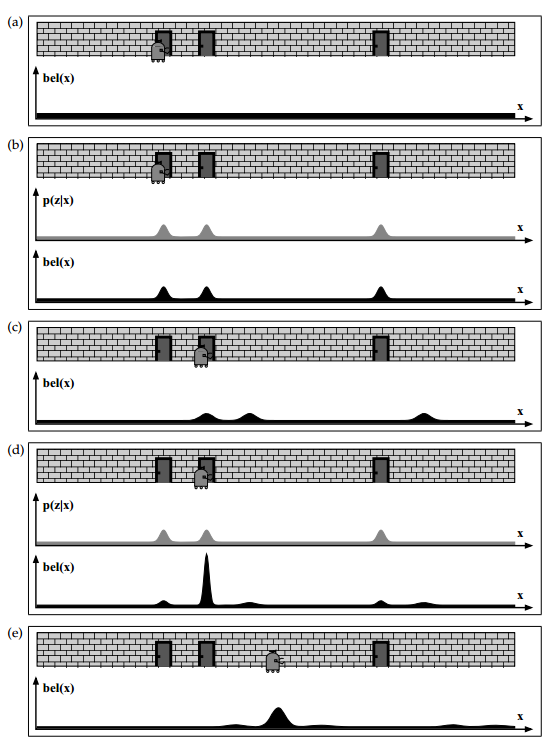
\includegraphics[width=0.8\linewidth]{figures/markovLocalization.png}
  \caption{Ý tưởng cơ bản của \textit{định vị Markov}: Robot di động đang định vị trong không gian toàn cục \cite{thrun2005probabilistic}}
  \label{fig:markovLocalization}
\end{figure}

Ví dụ thứ nhất là bài toán định vị robot di động. Định vị robot là ước tính vị trí tương đối của robot trong một không gian. Bản đồ của môi trường được cho trước, robot cần có các dữ liệu của cảm biến để tự định vị trong bản đồ này. Ví dụ về định vị được minh họa trong Hình \ref{fig:markovLocalization}. Môi trường đã biết có ba cửa giống nhau, nhiệm vụ của robot là tìm xem chúng ở đâu, thông qua cảm biến và chuyển động.

Vấn đề định vị cụ thể này được gọi là \textit{định vị toàn cục} (global localization). Trong định vị toàn cục, robot được đặt ở đâu đó trong một môi trường đã biết, nó phải tự định vị được vị trí của nó đang ở đâu. Mô hình xác suất thể hiện độ tin cậy tức thời của robot bằng một hàm phân bố xác suất trên toàn bộ không gian như trong \figurename{ \ref{fig:markovLocalization}}a. Biểu đồ này thể hiện phân bố đồng đều trên tất cả các vị trí. Bây giờ cho rằng robot nhận được dữ liệu đo đầu tiên từ cảm biến và theo dõi cánh cửa phía trước. Công cụ xác suất khai thác thông tin này để cập nhật vào độ tin cậy.
Độ tin cậy sau đó
% Cần sửa 'posterior belief% thể hiện trong
thể hiện trong \figurename{ \ref{fig:markovLocalization}}b, tăng xác suất tại vị trí gần các cửa và giảm xác suất ở vị trí khác.
Ta thấy rằng phân bố này có ba chóp giống nhau, mỗi chóp tương ứng với một cửa. Do đó robot không biết được nó đang ở đâu.

Bây giờ cho robot di chuyển, độ tin cậy đã được dịch chuyển theo hướng robot chuyển động (Thể hiện trong Hình \ref{fig:markovLocalization}c).
%Nó cũng trải ra một khoảng rộng hơn, thể hiện mức độ không chắc chắn thể hiện bởi sự dịch chuyển của robot.
Sự dịch chuyển của robot làm cho xác suất phân bố trong một khoảng rộng hơn.
\figurename{ \ref{fig:markovLocalization}d miêu tả độ tin cậy sau khi theo dõi một cửa khác.
Việc này dẫn đến thuật toán đặt phần lớn xác suất tại vị trí gần một cửa, và khi đó robot khá tự tin rằng nó đang ở đâu. Cuối cùng, \figurename{ \ref{fig:markovLocalization}}e thể hiện độ tin cậy của robot sau khi di chuyển một đoạn xa trong hành lang.

Ví dụ này minh họa một vài vấn đề của mô hình xác suất. Nói theo xác suất, việc quan sát của robot là một vấn đề ước tính trạng thái, ví dụ trên sử dụng một thuật toán có tên là \textit{bộ lọc Bayes} cho hậu ước tính qua không gian của định vị robot. Sử dụng một hàm phân bố xác suất để thể hiện thông tin. Việc cập nhật hàm phân bố này thể hiện thông tin thu được thông qua các phép đo của cảm biến, hoặc thông tin bị mất qua quá trình xử lý trong không gian làm tăng độ không chắc chắn của robot.

\begin{figure}[htbp]
  \centering
  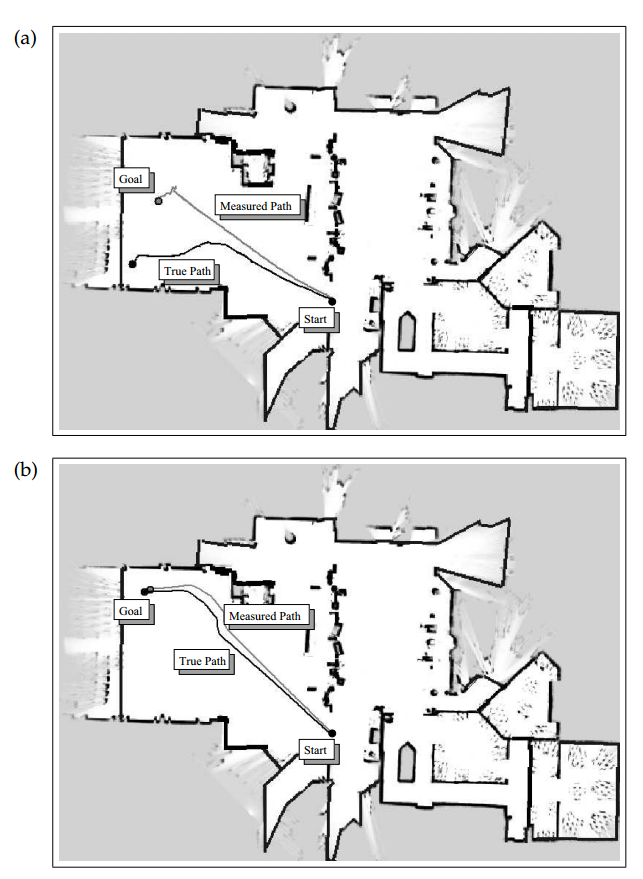
\includegraphics[width=0.8\linewidth]{figures/coastal-Navigation.png}
  \caption[Coastal navigation]{Hình (a): robot điều hướng qua môi trường mở, thiếu các đặc trưng trong không gian để có thể theo dõi được nó đang ở đâu (định vị). Hình (b): Vấn đề này có thể được tránh bằng việc đăt gần các vật cản đã biết. Hai hình này là kết quả của thuật toán \textit{coastal navigation} \cite{thrun2005probabilistic}}.
  \label{fig:coastalNavigation}
\end{figure}

Ví dụ thứ hai là một ví dụ trong vấn đề lập kế hoạch và điều khiển robot. Như đã nói các thuật toán xác suất có thể tính độ không chắc chắn tức thời của robot. Nhưng chúng cũng có thể đoán trước được độ không chắc chắn trong tương lai, và chọn một độ không chắc chắn để xem xét lựa chọn điều khiển. Một trong các thuật toán như vậy là \textit{coastal navitation}, ví dụ như trong \figurename{ \ref{fig:coastalNavigation}}. Hình này thể hiện một bản đồ 2-D của một tòa nhà. Hình phía trên so sánh đường đi ước tính và đường đi thực tế: robot đi lệch là kết quả của sự không chắc chắn trong chuyển động của robot. Điểm thú vị ở đây là không phải toàn bộ quỹ đạo có mức độ không chắc chắn như nhau. Đường đi trong \figurename{ \ref{fig:coastalNavigation}}a đi qua một không gian mở, thiếu các đặc trưng để có thể giúp cho robot định vị.  \figurename{ \ref{fig:coastalNavigation}}b có quỹ đạo bám theo một góc rõ ràng, và sau đó ôm vào tường để giữ định vị. Không quá ngạc nhiên khi mức độ không chắc chắn sẽ giảm sau một quãng di chuyển, do đó điểm đến có độ chính xác cao hơn.

Ví dụ này minh họa một trong những cách để xem xét ảnh hưởng của sự không chắc chắn trong điều khiển robot. Rõ ràng robot sẽ ưu tiên lựa chọn cách đi thứ hai hơn, dù có sự không chắc chắn nhưng thuật toán xác suất giúp robot lựa chọn đường đi để nó có thể thu thập được nhiều thông tin, giúp giảm độ không chắc chắn và đạt được độ chính xác tốt hơn.

% \subsection{Implications}
Xác suất trong robotics kết hợp không rõ ràng giữa mô hình và dữ liệu cảm biến, vượt qua các giới hạn của cả hai cùng lúc. Ý tưởng này không chỉ là vấn đề của điều khiển mức thấp, chúng có mặt tại mọi mức phần mềm robot từ thấp nhất tới cao nhất.

Trái ngược với các kĩ thuật lập trình truyền thống trong robot như các công cụ kế hoạch chuyển động dựa trên mô hình hay phản ứng dựa trên hành vi. Các cách tiếp cận theo xác suất có nhiều ưu điểm hơn với các giới hạn của cảm biến và mô hình hóa. Điều này giúp gần hơn với độ phức tạp của môi trường thế giới thực hơn là mô hình cũ. Trong thực tế, chắc chắn các thuật toán xác suất hiện nay chỉ mới biết các giải pháp với các vấn đề ước tính khó trong robotics như: vấn đề định vị, vấn đề xây dựng các bản đồ chính xác môi trường lớn.

So sánh với các công cụ robotics truyền thống dựa trên mô hình hóa, các thuật toán xác suất có yêu cầu thấp hơn về độ chính xác của các mô hình robot do đó giúp các nhà lập trình thoát khỏi gánh nặng không thể vượt qua để đưa ra các mô hình chính xác. Các thuật toán xác suất có yêu cầu thấp hơn về độ chính xác của các cảm biến hơn là các kĩ thuật dựa trên phản ứng, các kĩ thuật này phản ứng dựa trên dữ liệu cảm biến tức thời. Nhìn chung bài toán xác suất trong robot, việc học của robot là vấn đề ước lượng dài hạn.

Tuy nhiên, những ưu điểm này cũng đi liền với cái giá của nó. Hai hạn chế thường xuyên được nhắc tới đó là độ phức tạp tính toán và việc phải tính xấp xỉ. Các thuật toán xấp xỉ vốn đã kém hiệu quả hơn so với các thuật toán không xác suất. Do thuật toán này xem xét trên toàn bộ phân bố chứ không phải tại một lần đoán. Hầu hết các loại robot đều hoạt động liên tục yêu cầu các thuật toán này phải tính toán được theo thời gian thực. Một số bài toán có thể giải quyết bằng một số mô hình đơn giản (như Gaussians) nhưng một số bài toán khác yêu cầu phải có các mô hình phức tạp hơn.

Việc phát triển của phần cứng máy tính ngày nay làm tăng số lượng phép tính trên một đơn vị giá thành. Điều này giúp cho lĩnh vực xác suất robot có hiệu quả hơn, thực hiện được các bài toán khó hơn. Tuy nhiên vẫn còn đó thách thức tính toán của lĩnh vực này. \cite{thrun2005probabilistic}


\section{Hệ điều hành robot ROS và các ứng dụng}
%FIXME: 2 phần dưới đây có vẻ trùng nhau quá
\subsection{ROS là gì?}
Hệ điều hành Robot – Robot Operating System (ROS) là một nền tảng mã nguồn
mở phục vụ cho việc lập trình Robot, có thể cài đặt trên nhiều hệ điều hành khác
nhau như Windows, Linux hay Mac OS. ROS mang đến một nền tảng phần mềm
chung cho cộng đồng xây dựng và sử dụng Robot. Ở đó, mọi người có thể chia sẻ
các ý tưởng và các trình điều khiển dễ dàng hơn.
ROS đã đạt được rất nhiều thành tựu. Kể từ khi ra đời, đã có hơn 2000 các gói
phần mềm được viết và duy trì bởi gần 600 người. Gần 80 loại robot thương mại
được hỗ trợ và hàng nghìn các bài báo đề cập đến ROS. Chính vì thế, chúng ta đã
không còn phải làm tất cả mọi thứ từ đầu khi xây dựng Robot nhờ có sự trợ giúp
của ROS. Chúng ta có thể dành nhiều thời gian hơn để nghiên cứu về Robotics
thay vì tập trung quá nhiều vào xây dựng các trình điều khiển phần cứng.
ROS bao gồm tập hợp đa dạng các trình điều khiển cho phép chúng ta đọc dữ
liệu từ cảm biến, điều khiển các cơ cấu chấp hành; một lượng lớn các thuật toán
cho phép xây dựng bản đồ, điều hướng Robot, thu thập dữ liệu, lập kế hoạch di
chuyển\dots ROS cũng có một cộng đồng lớn nghiên cứu trong lĩnh vực Robot.

Nói cách khác, theo tác giả, ROS là một nền tảng cung cấp các phương thức để kết nối, trao đổi dữ liệu, quan sát dữ liệu giữa rất nhiều phần cứng với nhau như các cảm biến, các bộ phận chấp hành và các máy tính. Khi sử dụng ROS, người phát triển robot không cần quan tâm quá nhiều đến các thiết bị phần cứng (nếu thiết bị đó đã có thư viện driver ROS hỗ trợ), chỉ cần quan tâm đến việc tính toán, xử lý các dữ liệu để đạt được các mục đích trong các ứng dụng khác nhau. Nó làm giảm thời gian, giảm độ phức tạp khi phát triển robot đi rất nhiều lần.

\subsection{Tổng quan về HĐH ROS}
ROS là một nền tảng mã nguồn mở, một nền tảng phần mềm phục vụ cho việc
lập trình Robot. ROS cung cấp một hệ thống điều khiển phân tán cho các thiết bị
phần cứng khác nhau, được dùng để xây dựng các ứng dụng cho Robot mà không
cần phải quan tâm quá sâu về các phần cứng bên trong. ROS cung cấp các công cụ
đa dạng để mô phỏng, mô hình hóa Robot và xử lý dữ liệu của Robot, sử dụng giao
thức truyền thông tin đồng bộ hoặc không đồng bộ để liên kết và trao đổi dữ liệu
từ những thiết bị khác nhau.
Phần mềm được tổ chức thành các gói, rất thuận tiện, với giao thức truyền thông tin giữa các thiết bị phần cứng, nhà phát triển có thể tạo ra các mô hình robot
rất đa dạng, ví dụ như tạo bản đồ và điều hướng với robot di động. Các robot mới
có thể trực tiếp sử dụng các gói này mà không cần phải chỉnh sửa mã nguồn.
ROS cũng được sử dụng rộng rãi trong các trường Đại học, và có nhiều nhà phát
triển đóng góp. Có thể nói rằng, ROS có một cộng đồng lớn, có nhiều dự án được
hỗ trợ bởi cộng đồng phát triển toàn cầu. Có một hệ sinh thái thân thiện với các
mô hình phát triển Robot khác.
Tóm lại, ROS là sự kết hợp của mô hình truyền thông (Plumbing or
communication), các công cụ (Tools), khả năng phần cứng (Capabilities) và hệ
sinh thái (Ecosystem).

\begin{figure}[htbp]
  \centering
  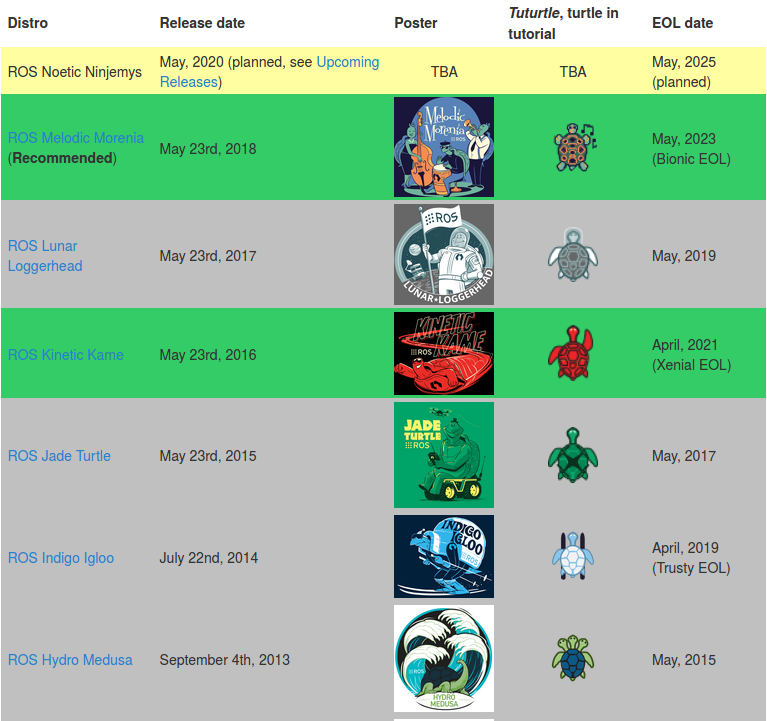
\includegraphics[width=0.9\linewidth]{figures/ROS-ditributions.png}
  \caption{Các bản phân phối gần đây của ROS \cite{wikiros}}
  \label{fig:ROS-distributions}
\end{figure}

\begin{figure}[htbp]
	\centering
	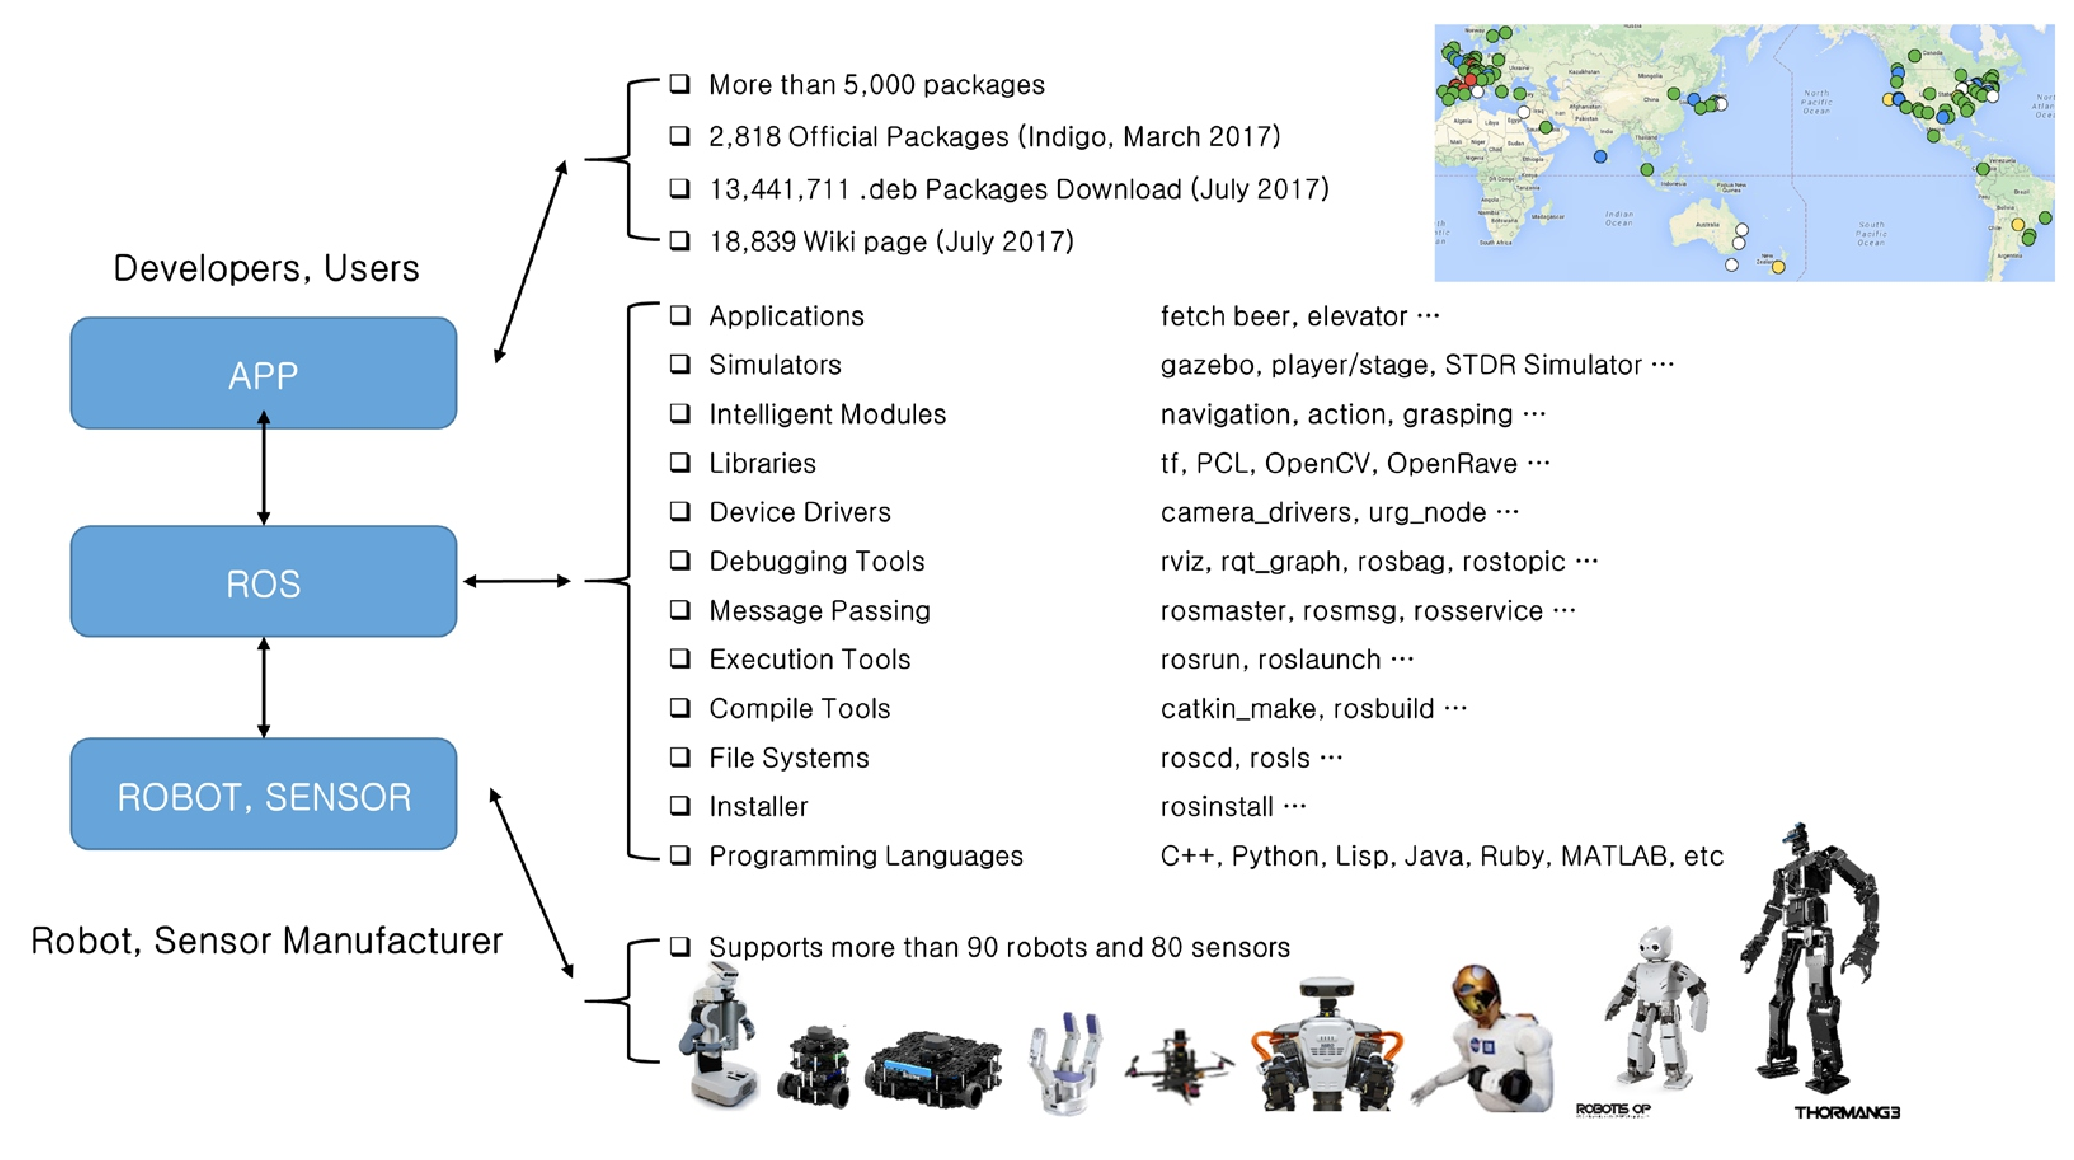
\includegraphics[width=1\linewidth]{figures/Ecosystem.pdf}
	\caption{Hệ sinh thái ROS \cite{pyo2017ros}}
	\label{fig:Ecosystem}
\end{figure}

ROS có nhiều bản phân phối khác nhau tương ứng với các bản phân phối của Linux và mỗi bản phân phối hỗ trợ cập nhật đến hết vòng đời. ROS tương thích hoàn toàn với hệ điều hành Ubuntu, phần lớn các bản phân phối của ROS được phát triển theo các phiên bản của Ubuntu \figurename{ \ref{fig:ROS-distributions}}

ROS như một hệ sinh thái, bao gồm từ các loại phần cứng thường dùng trong robot, các phần mềm, các nhà sản xuất và các nhà nghiên cứu \cite{wikiros}. \figurename{ \ref{fig:Ecosystem}} thể hiện hệ sinh thái ROS.


\subsection{Tại sao phải dùng ROS}

Hình dung rằng chúng ta đang xây dựng một robot tự hành thông minh. Chúng ta lựa chọn ROS hơn là các nền tảng robotic khác như Player, YARP, Orocos, MRPT... bởi các lý do như sau:
\begin{itemize}
	\item \textbf{Có độ sẵn sàng cao}: ROS có thể sử dụng được luôn, ví dụ như các gói thư viện SLAM (Simultaneous Localization and Mapping - tạm dịch là định vị và tạo bản đồ đồng thời) và AMCL(Adaptive Monte Carlo Localization - Là thuật toán định vị thích nghi Monte Carlo) trong ROS có thể được sử dụng cho robot di động di chuyển tự động và gói {\tt MoveIt} được sử dụng để lập kế hoạch chuyển động tay máy robot. Các gói thư viện này có thể dễ dàng sử dụng trực tiếp cho phần mềm robot của chúng ta. Việc sử dụng các gói thư viện này tốt hơn rất nhiều so với việc lập trình lại từ đầu để được thứ tương tự với một thứ đã có sẵn. Những gói chương trình này cũng rất dễ cấu hình lại, chúng ta có thể tinh chỉnh từng khả năng bằng cách sử dụng nhiều thông số khác nhau.
	\item \textbf{Rất nhiều công cụ}: ROS được đóng gói với rất nhiều công cụ để gỡ rối chương trình, hiển thị và mô phỏng các quá trình. Các công cụ như là {\tt rqt\_gui}, RViz, Gazebo là một số công cụ mã nguồn mở rất mạnh cho việc gỡ rối, hiển thị và mô phỏng.
	\item \textbf{Hỗ trợ cao cho các cảm biến và cơ cấu chấp hành}: ROS được đóng gói với các gói driver và giao tiếp với các thiết bị của rất nhiều cảm biến và cơ cấu chấp hành trong robotics. Các cảm biến cao cấp bao gồm Lidar, Laser scanners, Kinect... và các cơ cấu chấp hành như động cơ servo Dynamixel. Chúng ta rất dễ để có thể giao tiếp với các phần cứng này với ROS.
	\item \textbf{Khả năng phân tích nền tảng bên trong}: Việc truyền thông điệp (message) ROS ở tầng giữa cho phép giao tiếp giữa các node (node) với nhau. Các node này có thể đươc lập trình bằng bất kì ngôn ngữ nào có hỗ trợ thư viện ROS (như rospy trong python, roscpp trong C++). Chúng ta có thể viết các node trong C++ hoặc C và các node khác bằng Python hoặc Java. Điều này rất linh hoạt mà không có trong bất kì nền tảng nào khác.
	\item \textbf{Module hóa}: Một trong những các vấn đề có thể xảy ra trong phần lớn các ứng dụng robot đơn lẻ đó là, nếu bất kì luồng nào trong chương trình chính bị hỏng, toàn bộ ứng dụng robot đó có thể dừng lại. Trong ROS, trường hợp này sẽ khác, chúng ta viết các node khác nhau cho mỗi tiến trình và nếu một node bị hỏng, hệ thống vẫn có thể tiếp tục làm việc. ROS cũng cung cấp các phương pháp rất hữu ích để tiếp tục hoạt động một khi có bất kì cảm biến hoặc động cơ nào bị hỏng.
	\item \textbf{Điều khiển các nguồn tài nguyên đồng thời}: Việc sử dụng một nguồn tài nguyên phần cứng bởi nhiều hơn hai tiến trình luôn là một vấn đề đau đầu. Hãy hình dung, chúng ta muốn xử lý một hình ảnh từ một camera cho nhận dạng khuôn mặt và nhận dạng chuyển động, chúng ta có thể viết chương trình như một chương trình thực hiện toàn bộ cả hai vấn đề đó, hoặc chúng ta có thể viết riêng để thực hiện đồng thời. Nếu chúng ta muốn thêm nhiều hơn hai tính năng trong các luồng, hành vi ứng dụng sẽ trở nên phức tạp và rất khó để gỡ rối. Nhưng trong ROS, chúng ta có thể truy cập các thiết bị bằng cách sử dụng các chủ đề ROS từ các bộ điều khiển ROS (driver). Bao nhiêu node cũng có thể đăng kí tới thông điệp hình ảnh từ bộ điều khiển camera ROS và mỗi node có thể thực hiện các chức năng khác nhau. Nó có thể làm đơn giản tính toán và cũng như tăng khả năng gỡ rối của toàn bộ hệ thống.
	\item \textbf{Có một cộng đồng năng động}: Khi chúng ta lựa chọn một thư viện hoặc một nền tảng phần mềm, đặc biệt từ một cộng đồng mã nguồn mở, một trong những yếu tố chính là xem xét tới phần mềm hỗ trợ và cộng đồng các nhà phát triển sử dụng nó. Mã nguồn mở thì sẽ không đảm bảo có các công cụ hỗ trợ, một số công cụ có sự cung cấp hỗ trợ rất tốt nhưng ngược lại một số khác lại không. Trong ROS, cộng đồng hỗ trợ rất năng động. Có thể vào trang web sau để tham khảo sự hỗ trợ từ các người dùng khác: {\tt http://answers.ros.org}. Dường như cộng đồng ROS có sự tăng trưởng đều đặn của các nhà phát triển trên toàn thế giới.
\end{itemize}

Có rất nhiều lý do để lựa chọn ROS cho việc phát triển robot.

\subsection{Một số thành phần cơ bản trong ROS}

Một hệ thống ROS thông thường bao gồm những thành phần cơ bản như thể hiện trong \figurename{ \ref{fig:ros-filesystem}}.

\begin{figure}[htbp]
  \centering
  \begin{tikzpicture}[node distance=2cm]
    \node (no1) [process] {ROS Filesystem};
    \node (no2) [process, below of=no1, xshift=3.5cm] {Metapackages};
    \node (no3) [process, below of=no2, xshift=-3.5cm] {Packages};
    \node (no4) [process, below of=no3, xshift=-5cm] {Packages Manifest};
    \node (no5) [process, below of=no3, xshift=5cm] {Misc};
    \node (no6) [process, below of=no3, xshift=-3.2cm, node distance=4cm] {Messages};
    \node (no7) [process, below of=no3, xshift=0cm, node distance=4cm] {Services};
    \node (no8) [process, below of=no3, xshift=3.2cm, node distance=4cm] {Nodes};

    \draw [arrow] (no1) -- (no2);
    \draw [arrow] (no2) -- (no3);
    \draw [arrow] (no1) -- (no3);
    \draw [arrow] (no3)--++(-5,0) -- (no4);
    \draw [arrow] (no3)--++(5,0) -- (no5);
    \draw [arrow] (no3) --++(0,-0.5) -- (no6);
    \draw [arrow] (no3) --++(0,-1) -- (no7);
    \draw [arrow] (no3)--++(0,-0.5) -- (no8);

  \end{tikzpicture}
  \caption{ROS File System}
  \label{fig:ros-filesystem}
\end{figure}

Một số thuật ngữ, thành phần cơ bản trong ROS:

\textbf{Node} là đơn vị xử lý nhỏ nhất đang chạy trong ROS. Có thể coi nó như một chương trình thực thi. ROS khuyên rằng nên tạo một node đơn cho mỗi mục đích và nên phát triển để có thể dễ dàng sử dụng lại. Ví dụ, trong robot di động, chương trình để vận hành robot được chia thành các hàm chức năng nhỏ. Mỗi node được dùng cho một hàm chức năng như driver cảm biến, biến đổi dữ liệu cảm biến, nhận dạng vật cản, driver động cơ, đầu vào encoder và định hướng.

Khi khởi động, một node ghi thông tin như tên, dạng thông điệp, địa chỉ URI và số cổng của node. Node đã được ghi có thể hoạt động như một node xuất bản, node đăng kí, node chủ dịch vụ hoặc node khách dịch vụ dựa trên thông tin đã được ghi, và các node có thể trao đổi thông điệp bằng cách sử dụng chủ đề hoặc dịch vụ.

Node sử dụng XMLRPC cho việc giao tiếp với node chủ và sử dụng XMLRPC hoặc TCPROS của giao thức TCP/IP khi giao tiếp giữa các node với nhau. Yêu cầu kết nối và phản hồi giữa các node sử dụng XMLRPC và truyền thông điệp sử dụng TCPROS bởi vì nó là giao tiếp trực tiếp giữa các node với nhau mà không phụ thuộc vào node chủ. Với địa chỉ URI và số cổng, một biến được gọi là \codeword{ROS_HOSTNAME} được lưu trên máy tính, nơi node đang chạy, được sử dụng địa chỉ URI và cổng được đặt bằng một giá trị duy nhất bất kì.

\textbf{Master} có là một node đặc biệt, nó hoạt động như một máy chủ cho các kết nối node tới node và truyền thông điệp. Lệnh \codeword{roscore} được dùng để chạy node chủ, và nếu chạy node chủ, nó sẽ ghi tên của mỗi node và lấy thông tin khi cần thiết. Các hoạt động của ROS không được thực hiện khi chưa chạy master.

Giao tiếp giữa node chủ và các node khách bằng XMLRPC (Viết tắt của XML-Remote Produce Call: nghĩa là gọi hàm từ xa XML), là giao thức dựa trên HTTP không duy trì kết nối. Nói cách khác, các node khách chỉ có thể truy cập khi chúng cần ghi thông tin của chúng hoặc yêu cầu thông tin của các node khác. Trạng thái kết nối không được kiểm tra thường xuyên. Vì đặc điểm này, ROS có thể được sử dụng trong các môi trường rất lớn và phức tạp. XMLRPC rất nhẹ và hỗ trợ rất nhiều ngôn ngữ lập trình khác nhau, rất phù hợp để sử dụng cho ROS vì ROS hỗ trợ rất nhiều phần cứng và nhiều ngôn ngữ lập trình.
\textbf{Packages:} Gói chương trình là đơn vị chính trong tổ chức phần mềm của hệ điều hành ROS. Một package có thể chứa các lệnh thực thi của ROS (các node), thư viện, các tệp chứa thông số\dots Package chính là thành phần nguyên tử nhỏ nhất được xây dựng và đưa vào sử dụng trong ROS.

\textbf{Packages Manifest:} Bảng kê khai thông tin dữ liệu của package (package.xml), cung cấp siêu dữ liệu về package đó bao gồm tên gọi, phiên bản, thông tin bản quyền (license) và những yếu tố phụ thuộc của gói dữ liệu đó. Manifest còn chứa thông tin về đặc trưng của ngôn ngữ lập trình ví dụ như các cờ báo (flags) của trình biên dịch.

\textbf{Message} hay còn gọi là thông điệp, thông tin. Một node gửi hoặc nhận dữ liệu giữa các node thông qua một thông điệp. Các thông điệp là cá biến như số nguyên (integer), điểm số thực (floating point), hay logic (boolean). Có thể sử dụng thông điệp lồng vào các thông điệp hoặc một mảng các thông điệp khác.

Giao thức truyền thông TCPROS và UDPROS được sử dụng để truyền thông điệp. Chủ đề (topic) được sử dụng để truyền thông điệp đơn hướng trong khi dịch vụ (service) được dùng để truyền thông điệp đa hướng bao gồm yêu cầu và phản hồi.

\textbf{Truyền thông tin: } ROS được phát triển dựa trên các đơn vị node, đơn vị nhỏ nhất để thực thi các chương trình đã chia nhỏ để có thể dễ dàng tái sử dụng theo các mục đích. Node trao đổi dữ liệu với nhau thông qua thông điệp message để tạo thành một chương trình lớn. Các node sẽ giao tiếp với nhau bằng cách trao đổi các thông điệp. Thông điệp có thể là các kiểu dữ liệu đơn giản như số nguyên, số thực, kí tự, biến logic… hoặc cũng có thể là tổ hợp của các thông điệp khác như: tọa độ của một điểm là tổ hợp của 3 số thực. Trong thực tế, ROS có rất nhiều loại thông điệp từ đơn giản đến phức tạp để phục vụ cho việc xử lí dữ liệu đa dạng, ví dụ như: thông điệp hình ảnh, thông điệp là dữ liệu từ một cảm biến, thông điệp là vị trí và vận tốc của robot…
Có 3 phương pháp để trao đổi dữ liệu: \codeword{topic, service, action}. Ngoài ra, các thông số được sử dụng trong node có thể được thay đổi từ bên ngoài node. Điều này có thể được xem như một dạng của sự truyền thông điệp với nội dung lớn hơn. Sự truyền thông điệp được mô tả trong \figurename{ \ref{fig:messageCommunication}}

\begin{figure}[htbp]
  \centering
  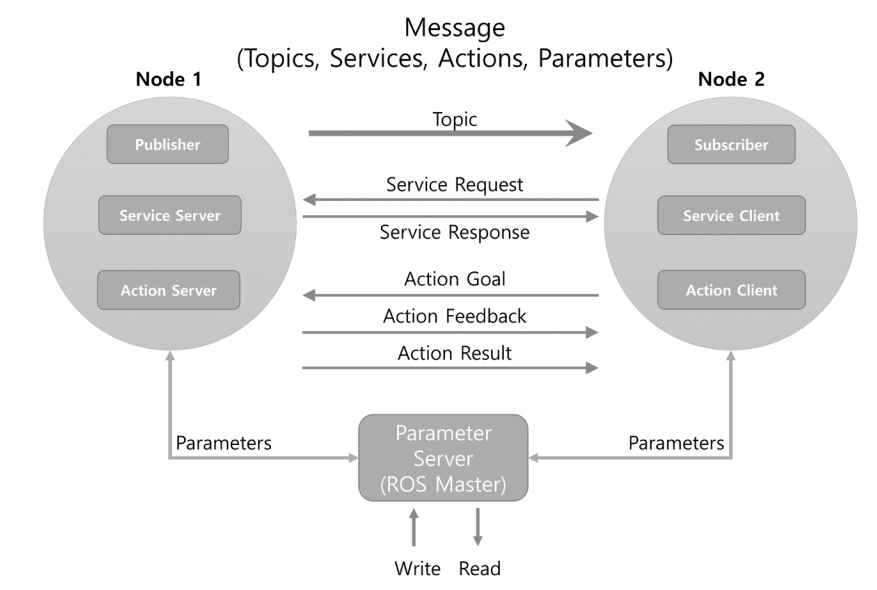
\includegraphics[width=0.8\linewidth]{figures/messageCommunication.png}
  \caption{Truyền thông giữa hai node}
  \label{fig:messageCommunication}
\end{figure}

\begin{figure}[htbp]
  \centering
  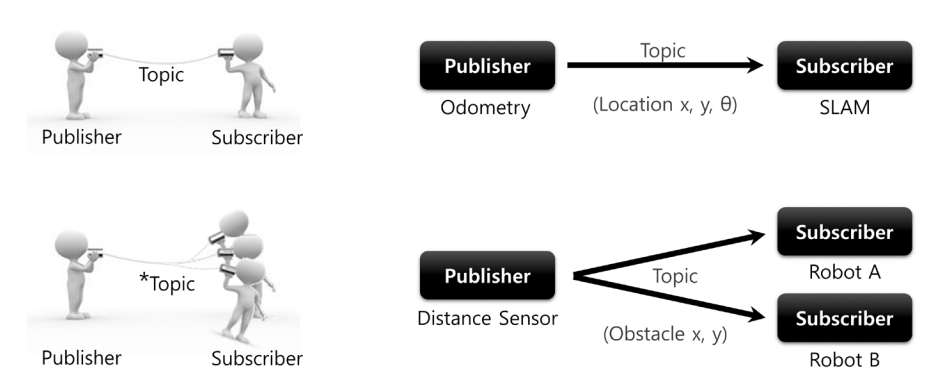
\includegraphics[width=0.9\linewidth]{figures/topic.png}
  \caption{Kiểu giao tiếp topic}
  \label{fig:topic}
\end{figure}

\textbf{Topic} hay còn gọi là chủ đề, giống như nghĩa đen là chủ đề trong một đoạn hội thoại. Node xuất bản đầu tiên ghi thông tin chủ đề của nó với node chủ và sau đó bắt đầu xuất bản thông điệp trên một chủ đề. Các node đăng kí muốn nhận chủ đề yêu cầu thông tin của node đăng kí khớp với tên của chủ đề đã được ghi ở trên node chủ. Dựa vào thông tin này, node đăng kí kết nối trực tiếp tới node xuất bản để trao đổi thông điệp như một chủ đề. \figurename{ \ref{fig:topic}}

\textbf{Publish và Publisher} Hay còn gọi là xuất bản và node xuất bản. Xuất bản là thuật ngữ dành cho hành động chuyển các thông điệp liên quan tới đúng chủ đề. Node xuất bản ghi thông tin của nó và chủ đề với node chủ, và gửi một thông điệp tới các node đăng kí, là các node quan tâm tới cùng chủ đề.
\textbf{Subscribe và Subscriber:} Thuật ngữ 'Subscribe', còn gọi là Đăng kí, thể hiện hành động của việc nhận các thông điệp khớp với topic. Node Subscriber đăng kí thông tin của nó và chủ đề với master, và nhận thông tin của các node xuất bản.

\begin{figure}[htbp]
  \centering
  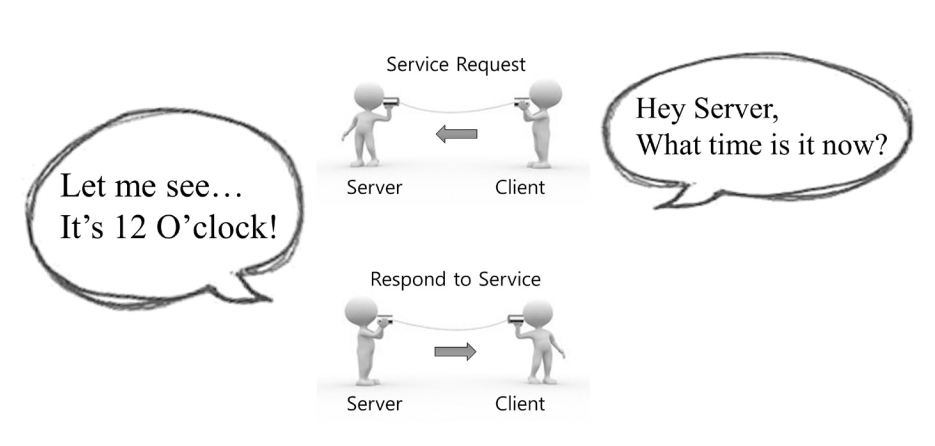
\includegraphics[width=0.9\linewidth]{figures/service.png}
  \caption{Kiểu giao tiếp service}
  \label{fig:service}
\end{figure}
\textbf{Service: } Giao tiếp đồng bộ giữa dịch vụ khách (service client) và máy chủ dịch vụ (service server). Khách sẽ yêu cầu (request) 1 dịch vụ và máy chủ dịch vụ sẽ phản hồi lại yêu cầu đó. Khác với mô hình xuất bản - đăng kí, là một phương pháp không đồng bộ gặp khó khăn trong các phương pháp truyền dữ liệu theo chu kỳ, mô hình yêu cầu and phản hồi là 1 phương pháp đồng bộ, trong trường hợp này là Service \figurename{ \ref{fig:service}}.

\begin{figure}[htbp]
  \centering
  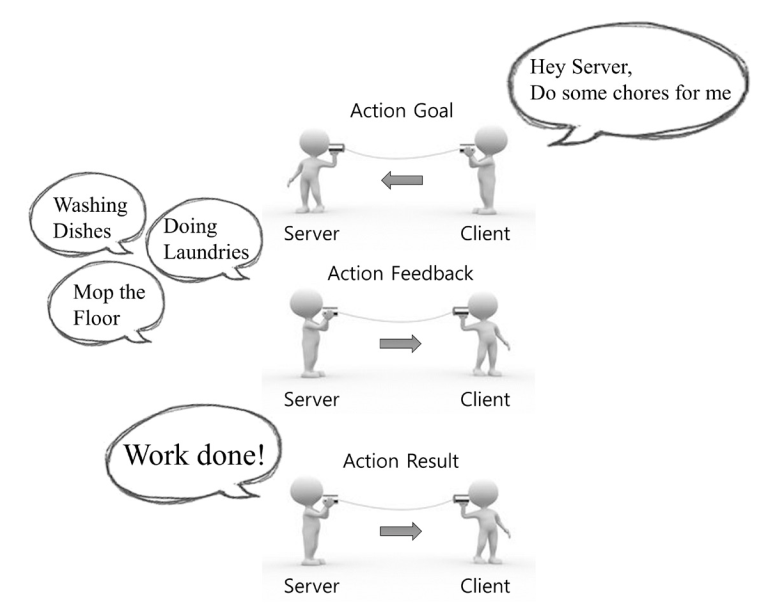
\includegraphics[width=0.8\linewidth]{figures/action.png}
  \caption{Kiểu giao tiếp Action}
  \label{fig:action}
\end{figure}
\textbf{Action:} Được sử dụng khi một nhiệm vụ thực hiện cần nhiều thời gian để hoàn thành cần 1 quá trình phản hồi (feedback). Trong action, \codeword{goals} và \codeword{results} sẽ tương tự như \codeword{request} (yêu cầu) và \codeword{response}(đáp ứng), ngoài ra còn có thêm \codeword{feedback} là tín hiệu phản hồi đến khách theo chu kì


\section{Bài toán điều hướng robot }

  % Tóm gọn nội dung giới thiệu về ROS và các ứng dụng trong khuôn khổ của luận văn này.

  Giống như chúng ta sử dụng GPS để định vị và tìm đường trong quá trình di chuyển giữa thành phố đông đúc, rộng lớn, hoặc khi ta đi tới một địa điểm xa lạ. Khi đó chúng ta sử dụng các ứng dụng trên điện thoại di động như googlemap để định vị vị trí của mình, sau đó tìm đường tới địa điểm mong muốn. Tương tự như vậy, robot tự hành cũng cần định vị, và xác định đường đi tới điểm đích.

\subsection{Điều hướng robot di động}

Điều hướng không thể thiếu trong robotics. Điều hướng là sự di chuyển của robot tới một đích xác định, điều này không dễ dàng với robot. Robot phải biết được nó đang ở đâu và phải có một bản đồ của môi trường. Robot phải tìm được đường đi tối ưu trong rất nhiều đường đi khác, tránh vật cản như tường, đồ vật. Để có thể điều hướng robot, cần những yếu tố sau:
\begin{itemize}
  \item Bản đồ
  \item Trạng thái của robot\footnote{Trong luận văn này, khi nhắc đến trạng thái robot có nghĩa là vị trí và hướng của robot}
  \item Cảm nhận thông tin từ cảm biến
  \item Tính toán đường đi và di chuyển
\end{itemize}

\subsubsection*{Bản đồ}
Tương tự như hệ thống điều hướng trên các phương tiện, hay ứng dụng google map chúng ta sử dụng hằng ngày đều có bản đồ rất chính xác và được cập nhật thường xuyên. Còn với robot, chúng cũng cần có bản đồ. Vì vậy chúng ta sẽ phải tạo một bản đồ và cung cấp cho nó, hoặc robot có thể tự tạo bản đồ.

SLAM (Simultaneous Localization And Mapping) được phát triển để robot có thể tự nó khám phá và tạo bản đồ tại một môi trường chưa biết.

\subsubsection*{Trạng thái của robot}
Robot cần phải đo và ước tính được trạng thái của nó. Hiện nay, phương pháp được sử dụng rộng rãi nhất để ước tính trạng thái trong nhà cho robot dịch vụ là \codeword{dead reckoning}\footnote{\url{https://en.wikipedia.org/wiki/Dead_reckoning}} - dùng để ước tính trạng thái robot, nhưng nó đã được sử dụng từ rất lâu và phù hợp với các cảm biến giá rẻ và có thể đạt được một độ chính xác nhất định. Sự dịch chuyển của robot được đo bằng số vòng quay của bánh xe. Tuy nhiên, có sai số giữa khoảng cách tính được với số vòng quay của bánh xe và khoảng cách dịch chuyển thực tế. Tuy nhiên, thông tin quán tính từ IMU có thể được sử dụng để giảm thiểu sai số bằng việc bù sai số của vị trí và hướng giữa giá trị tính được và giá trị thực tế.

\begin{figure}
\centering
\subfloat[][]{
\label{fig:mobile-rb-dead-reckoning}
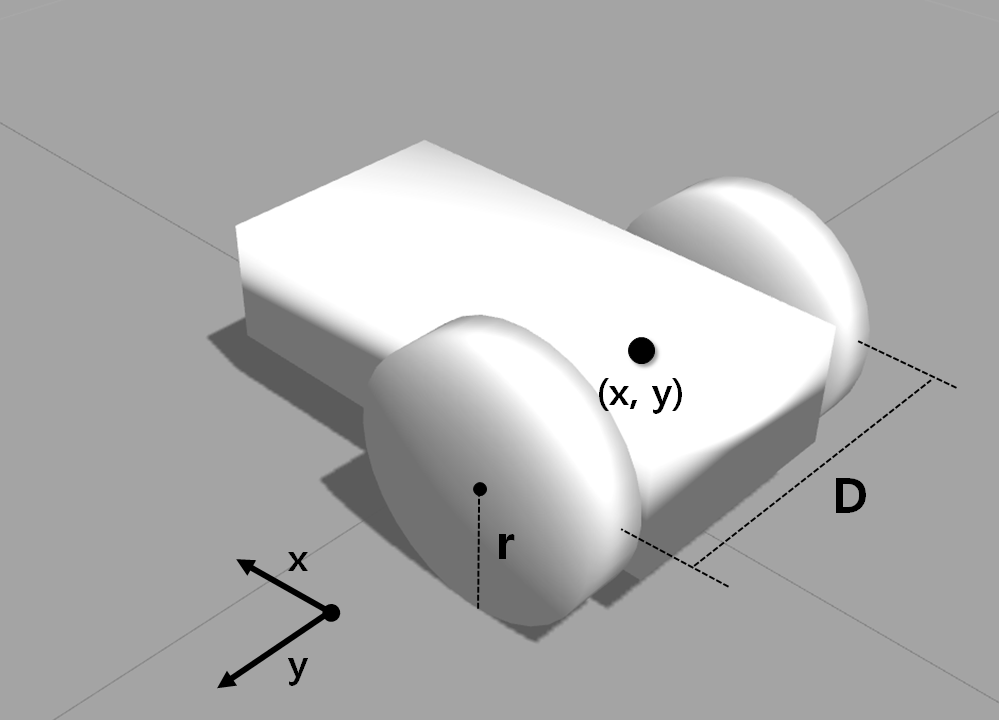
\includegraphics[width=0.3\textwidth]{figures/mobile-rb-dead-reckoning.png}}
\subfloat[][]{
  \label{fig:dead-reckoning}
  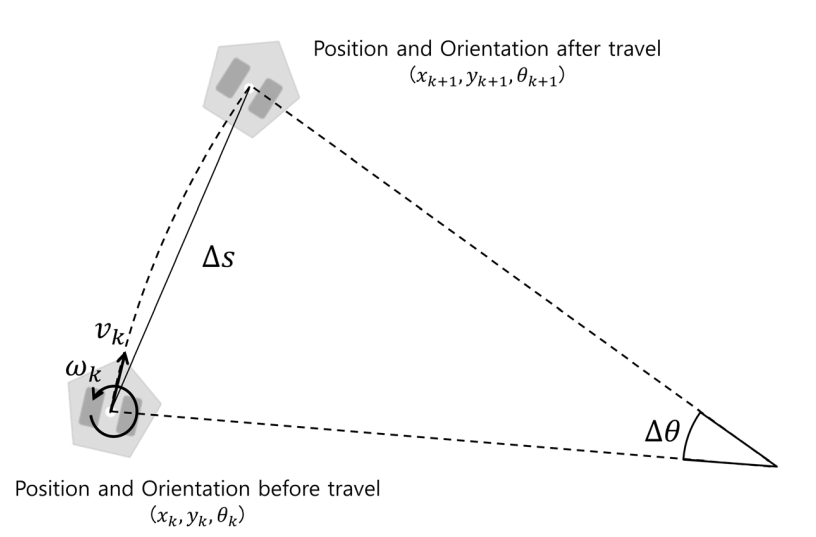
\includegraphics[width=0.6\textwidth]{figures/dead-reckoning.png}}
  \caption{Dead Reckoning}
  \label{fig:deadReckoning}
\end{figure}

\figurename{ \ref{fig:mobile-rb-dead-reckoning}} thể thông tin cần thiết cho dead reckoning
bao gồm tọa độ tâm robot (x,y), khoảng cách giữa hai bánh xe D và bán kính bánh r.
% \figurename{ \ref{fig:dead-reckoning}} là mô hình dead reckoning.
Giả sử robot di chuyển một đoạn ngắn trong khoảng thời gian ${T}_{e}$, vận tốc góc $({v}_{l}, {v}_{r})$ của bánh trái và bánh phải được tính như trong phương trình \ref{equa:deadReckoning-vl} và \ref{equa:deadReckoning-vr} với góc quay của động cơ bên trái và bên phải (giá trị encoder hiện tại là ${E}_{l}c, {E}_{r}c$ và giá trị encoder trước đó là ${E}_{r}p, {E}_{l}p$)

\begin{equation}
  {v}_{l} = \frac{({E}_{l}c - {E}_{l}p)}{{T}_{e}}.\frac{\pi}{180}  (rad/s)
  \label{equa:deadReckoning-vl}
\end{equation}
\begin{equation}
  {v}_{r} = \frac{({E}_{r}c - {E}_{r}p)}{{T}_{e}}.\frac{\pi}{180}  (rad/s)
  \label{equa:deadReckoning-vr}
\end{equation}

Phương trình \ref{equa:V_l} và \ref{equa:V_r} tính vận tốc của bánh trái và bánh phải $({V}_{l}, {V}_{r})$. Từ vận tốc bánh trái và bánh phải, vận tốc dài (${v}_{k}$) và vận tốc góc (${\omega}_{k}$) của robot có thể tính được như phương trình \ref{equa:v_k} và \ref{equa:omega_k}

\begin{equation}
  {V}_{l} = {v}_{l}.r (m/s)
  \label{equa:V_l}
\end{equation}
\begin{equation}
  {V}_{r} = {v}_{r}.r (m/s)
  \label{equa:V_r}
\end{equation}
\begin{equation}
  {v}_{k} = \frac{({V}_{r}+{V}_{l})}{2} (m/s)
  \label{equa:v_k}
\end{equation}
\begin{equation}
  {\omega}_{k} = \frac{({V}_{r}-{V}_{l})}{D} (rad/s)
  \label{equa:omega_k}
\end{equation}

Cuối cùng, sử dụng những giá trị này, chúng ta có thể tính được vị trí (${x}_{(k+1)},{y}_{(k+1)}$) và hướng ${\theta}_{k+1}$ của robot từ phương trình \ref{equa:delta} tới phương trình \ref{equa:theta_k}

\begin{equation}
  {\Delta}s = {v}_{k}{T}_{e} \qquad
  {\Delta}{\theta} = {\omega}_{k}{T}_{e}
  \label{equa:delta}
\end{equation}
\begin{equation}
  {x}_{k+1} = {x}_{k} + {\Delta}s .{\cos} \left( {\theta}_{k}+\frac{{\Delta}{\theta}}{2} \right)
  \label{equa:x_kp1}
\end{equation}
\begin{equation}
  {y}_{k+1} = {y}_{k} + {\Delta}s .{\sin} \left( {\theta}_{k}+\frac{{\Delta}{\theta}}{2} \right)
  \label{equa:y_kp1}
\end{equation}
\begin{equation}
  {\Theta}_{k+1} = {\theta}_{k} + {\Delta}{\theta}
  \label{equa:theta_k}
\end{equation}

\subsection*{Cảm nhận môi trường}
Thứ ba, việc phát hiện ra đâu là vật cản như tường, các đồ vật yêu cầu cần có các cảm biến. Có nhiều loại cảm biến như cảm biến khoảng cách và cảm biến hình ảnh. Cảm biến khoảng cách dạng laser như LDS, LRF, LiDAR, cảm biến siêu âm và cảm biến hồng ngoại. Cảm biến hình ảnh bao gồm stereo camera, monocamera, omnidirectional camera,\dots và hiện nay có các loại camera như RealSense, Kinect, Xtion được sử dụng rộng rãi như camera chiều sâu để phát hiện các vật cản.

\subsection*{Tính toán đường đi và di chuyển}
Một đặc điểm cuối cùng cho điều hưởng robot là tính toán và di chuyển theo đường đi tối ưu từ vị trí hiện tại tới đích xác định trong bản đồ. Được gọi là tìm kiếm đường đi và lên kế hoạch di chuyển. có nhiều thuật toán như thuật toán ${A}^{*}$, thuật toán \textit{trường tiềm năng}(Potential Field), \textit{Lọc từng phần} (particle filter)\dots

Kế hoạch di chuyển bao gồm cả \textit{kế hoạch đường đi toàn cục} (global path planning) trên toàn bộ bản đồ và \textit{kế hoạch đường đi địa phương} (local path planning) cho một vùng nhỏ hơn xung quanh robot.

\subsection*{Di chuyển và tránh vật cản}
Nếu một lệnh gửi tới robot trên quỹ đạo di chuyển được tạo bằng \textit{kế hoạch chuyển động} (motion planing), robot di chuyển tới đích theo đường đi đã được lên kế hoạch. Do đó việc cảm nhận môi trường, ước tính trạng thái vị trí robot và kế hoạch chuyển động vẫn tiếp tục thực hiện, tính toán trong quá trình di chuyển., các vật cản và đối tượng di động mới xuất hiện trong môi trường sẽ được phát hiện và tránh bởi giải thuật \textit{Cửa sổ tiếp cận động} (Dynamic Window Approach - DWA).

\subsection{Bản đồ trọng số (costmap)}

Trạng thái của robot được ước tính dựa trên odometry từ encoder và cảm biến gia tốc góc IMU. Và khoảng cách giữa robot và các vật cản được tính từ cảm biến khoảng cách gắn trên robot. Trạng thái robot và cảm biến, thông tin vật cản, một bản đồ lưới chiếm dụng là kết quả của SLAM được sử dụng để tải bản đồ tĩnh và sử dụng các vùng bị chiếm dụng, các vùng trống và các vùng chưa biết cho điều hướng robot.

Trong điều hướng robot, bản đồ trọng số tính vùng có vật cản, các vùng có khả năng va chạm và vùng robot có thể di chuyển. Phụ thuộc vào kiểu điều hướng, bản đồ trọng số có thể chia thành hai phần. Một là \textit{global\_costmap}, thiết lập kế hoạch di chuyển cho điều hướng robot trong toàn bộ không gian của bản đồ cố định. Phần còn lại là \textit{local\ costmap} được sử dụng cho kế hoạch di chuyển và tránh vật cản trong không gian giới hạn quanh robot. Mặc dù mục đích khác nhau nhưng cả hai loại bản đồ này được thể hiện theo cùng một cách.

\begin{figure}[htbp]
  \centering
  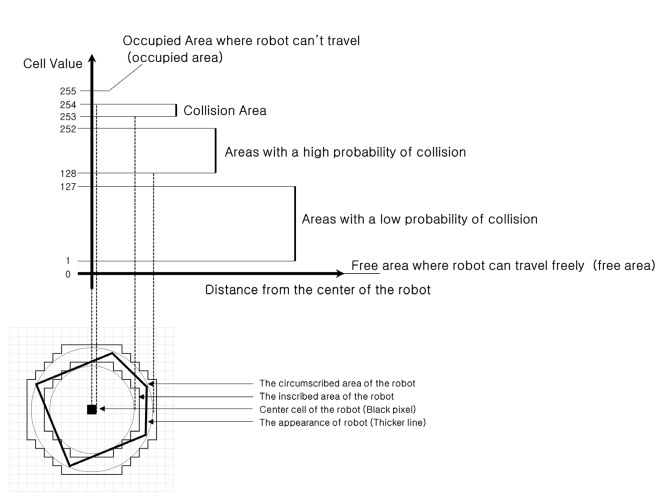
\includegraphics[width=0.8\linewidth]{figures/relationship-distanceToObstacle-vs-costmapValue.png}
  \caption{Quan hệ giữa khoảng cách tới vật cản và giá trị bản đồ trọng số}
  \label{fig:relationship-distanceToObstacle-vs-costmapValue}
\end{figure}

Bản đồ trọng số thể hiện giá trị từ 0 tới 255. Nghĩa của từng giá trị được thể hiện trong \figurename{ \ref{fig:relationship-distanceToObstacle-vs-costmapValue}, và tóm tắt như sau, được dùng để xác định nơi robot có thể di chuyển hoặc va chạm với vật cản.

\begin{itemize}
  \item \textbf{000:} vùng trống robot có thể di chuyển thoải mái
  \item \textbf{001 - 127}: vùng xác suất thấp có vật cản
  \item \textbf{128 - 252}: vùng xác suất cao có vật cản
  \item \textbf{253 - 254}: vùng có vật cản
  \item \textbf{255}: vùng bị chiếm dụng, robot không thể di chuyển.
\end{itemize}

\subsection{AMCL}
AMCL (Adaptive Monte Carlo Localization) có thể xem như phiên bản nâng cấp của phương pháp ước tính trạng thái vị trí Monte Carlo, cái thiện hiệu suất thời gian thực bằng cách giảm thời gian tính toán với số mẫu nhỏ hơn giải thuật Monte Carlo.
Mục đích của giải thuật ước tính trạng thái vị trí Monte Carlo (MCL) là xác định vị trí robot trong môi trường đã biết, đó là $x$, $y$ và $\theta$ của robot trong bản đồ.
MCL tính xác suất nơi robot có thể được đặt. Đầu tiên, vị trí và hướng ($x, y, \theta$) của robot tại thời điểm t được biểu thị là ${x}_{t}$,
và thông tin khoảng cách từ cảm biến tới thời điểm t được biểu thị là ${z}_{0..t} = \left\{{z}_{0}, {z}_{1}, ..., {z}_{t}\right\}$, và thông tin di chuyển từ encoder tới thời điểm t là ${u}_{0..t} = \left\{{u}_{0}, {u}_{1}, ..., {u}_{t}\right\}$. Chúng ta có thể tính độ tin cậy với phương trình:
\begin{equation}
  bel({x}_{t} = p\left({x}_ {t}|{z}_{0..t}, {u}_{0..t}\right))
\end{equation}

Vì robot có thể có sai số phần cứng nên phải thiết lập mô hình cảm biến và mô hình di chuyển. Áp dụng quá trình dự đoán và cập nhật của bộ lọc Bayes.

Trong bước dự đoán, vị trí $bel'\left({x}_{t}\right)$ của robot tại thời gian tiếp theo được tính bằng cách sử dụng mô hình di chuyển $p\left({x}_ {t}|{z}_{0..t}, {u}_{0..t}\right)$ của robot và xác suất $bel({x}_{t}$ tại vị trí trước đó, và thông tin chuyển động $u$ nhận được trước đó.

\begin{equation}
  bel'({x}_{t} = \int p\left({x}_ {t}|{z}_{0..t}, {u}_{0..t}\right))bel\left({x}_{t-1}\right)d{x}_{t-1}
\end{equation}

Tiếp theo là bước cập nhật. Thời điểm này, mô hình cảm biến $p\left({z}_{t}|{x}_{t}\right)$, xác suất $bel\left({x}_{t}\right)$ và hằng số chuẩn $\left({\eta}_{t}\right)$ được dùng để nâng độ chính xác xác suất $bel'\left({x}_{t}\right)$ dựa trên thông tin cảm biến.

\begin{equation}
  bel({x}_{t}) = {\eta}_{t} p\left({z}_ {t}|{x}_{0..t}\right)bel'({x}_{t})
\end{equation}

Phương trình sau để ước tính vị trí bằng việc tạo ra N điểm mẫu với particle filter sử dụng các xác suất đã tính $bel({x}_{t})$ của vị trí hiện tại. Đầu tiên là quá trình lấy mẫu. Ở đây, có một tập mẫu ${x}_{t}'$ được trích xuất bằng cách sử dụng mô hình di chuyển của robot $p\left({x}_{t}|{x}_{t-1}, {u}_{t-1}\right)$ tại xác suất $bel({x}_{t-1})$ của vị trí trước. Mẫu thứ \textit{i} ${{x}_{i}'}^{(i)}$ giữa tập mẫu ${x}_{t}'$, thông tin khoảng cách ${z}_{t}$ và hằng số chuẩn hóa $\eta$ được sử dụng để tính trọng số ${\omega}_{t}^{(i)}$.

\begin{equation}
  {\omega}_{t}^{(i)} = {\eta}p\left({z}_{t}|{x}_{t}'^{(i)}\right)
\end{equation}

Cuối cùng, trong quá trình lấy mẫu lại, chúng ta tạo N mẫu mới ${X}_{t}$ sử dụng mẫu ${{x}_{t}'}^{(i)}$ và trọng số ${\omega}_{t}^{(i)}$.

\begin{equation}
  X_t = \left\{x_t^{(j)} | j = 1..N\right\} ~  \left\{x_t'^{(i)}, {\omega}_t^{i}\right\}
\end{equation}

Bằng việc lặp lại quá trình trên trong khi di chuyển các điểm mẫu, vị trí được ước tính của robot có độ chính xác tăng lên. Ví dụ như trong \figurename{ \ref{fig:AMCLprocess}}, quá trình hội tụ vị trí từ 't1' tới 't4'. Tất cả quá trình này đã được mô tả trong phần \ref{subsec:probabilityinRobotics}. \cite{pyo2017ros}

\begin{figure}[htbp]
  \centering
  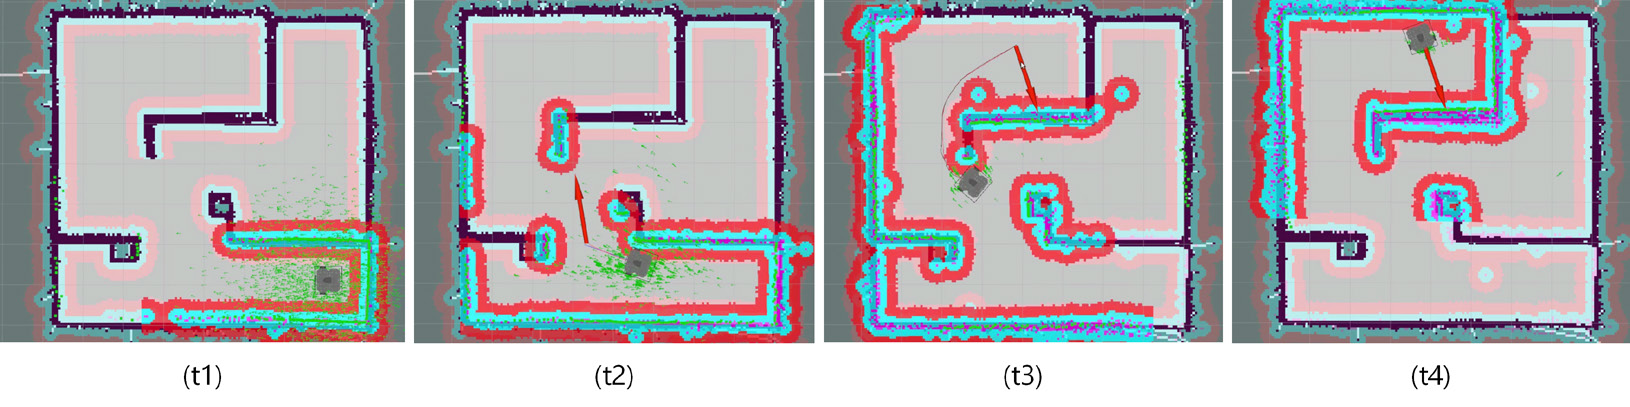
\includegraphics[width=1\linewidth]{figures/AMCL-process-for-pose-estimate.png}
  \caption{Quá trình AMCL cho ước tính trạng thái vị trí robot}
  \label{fig:AMCLprocess}
\end{figure}

\subsection{Cửa sổ tiếp cận động (Dynamic Window Approach - DWA)}
DWA là phương pháp phổ biến cho di chuyển và tránh vật cản. Đây là phương pháp lựa chọn tốc độ để có thể tới điểm đích nhanh nhất trong khi tránh vật cản. Trong ROS, \codeword{Trajectory planner} được dùng để tạo kế hoạch di chuyển cục bộ, nhưng DWA được dùng để thay thế vì sự vượt trội của nó.

Đầu tiên, robot không nằm trong hệ tọa độ x, y mà trong không gian tìm kiếm với tốc độ di chuyển $x$ và vận tốc góc $\omega$, như trong \figurename{ \ref{fig:dwa}}. Trong không gian này, robot có tốc độ tối đa cho phép do giới hạn phần cứng và được gọi là Cửa sổ động.

Trong cửa sổ động này, hàm mục tiêu $G(v, \omega)$ được dùng để tính vận tốc dài x và vận tốc góc $\omega$ tối đa từ hàm mục tiêu trên và xem xét hướng, vận tốc và vật cản của robot. Nếu vẽ đồ thị ra chúng ta có thể tìm được vận tốc tối ưu giữa nhiều giá trị $v$ và $\omega$ để tới đích như trong \figurename{ \ref{fig:dwa-search-velocity}}

\begin{figure}[htbp]
  \centering
  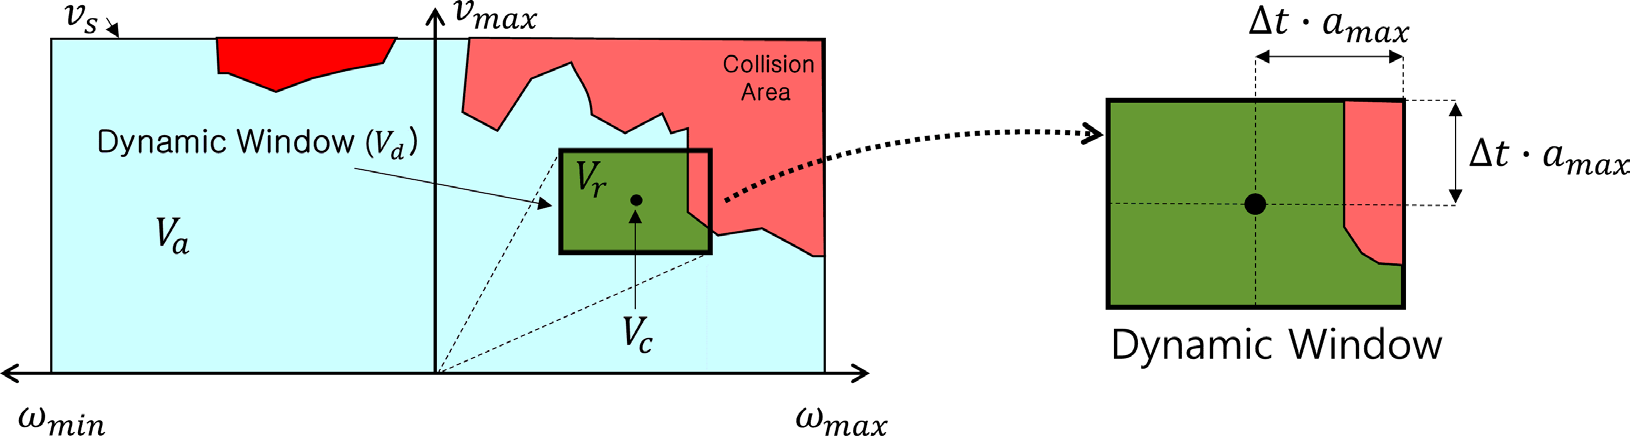
\includegraphics[width=1\linewidth]{figures/DWA.png}
  \caption{Không gian tìm kiếm vận tốc và cửa sổ động}
  \label{fig:dwa}
\end{figure}

\begin{figure}[htbp]
  \centering
  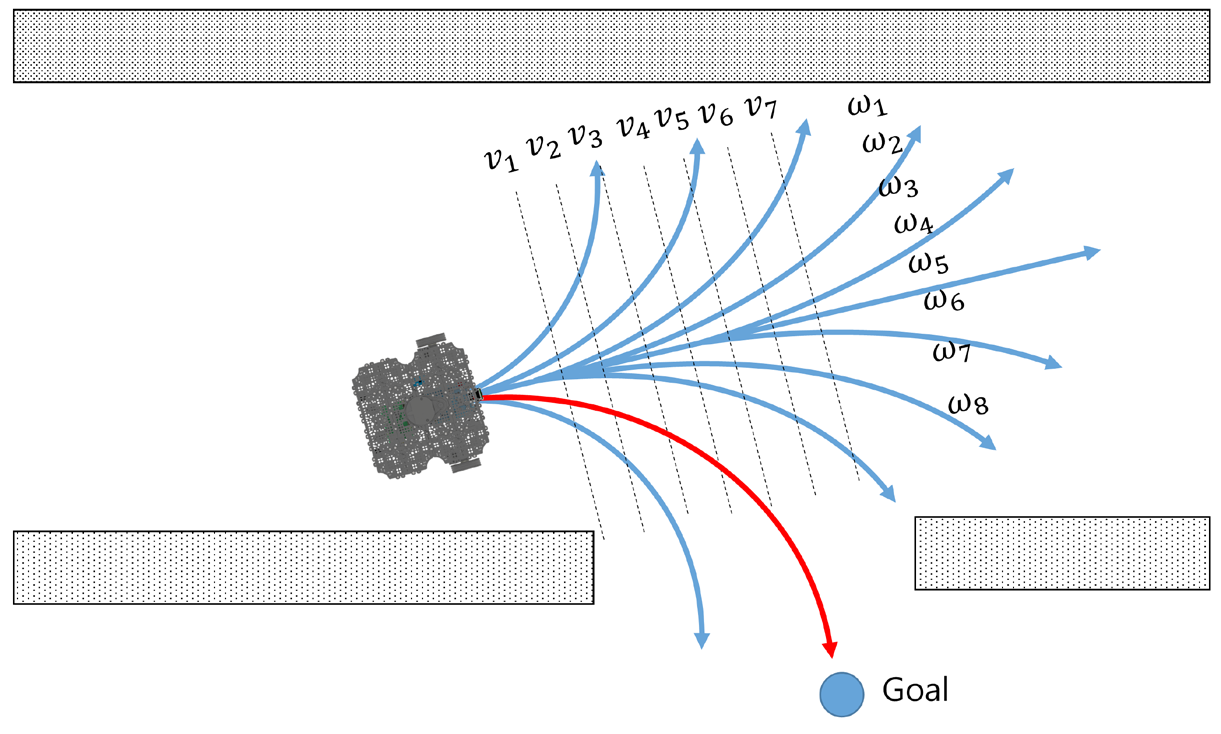
\includegraphics[width=0.8\linewidth]{figures/dwa-search-velocity.png}
  \caption{Vận tốc dài v và vận tốc góc $\omega$}
  \label{fig:dwa-search-velocity}
\end{figure}

% \section{Bài toán SLAM 2D}
\section{Bài toán định vị và tạo bản đồ đồng thời}

% \subsection{SLAM}

% SLAM(Simultaneus Localization And Mapping) có nghĩa là khám phá và tạo bản đồ của một môi trường chưa biết trong khi ước tính trạng thái vị trí của chính nó bằng dữ liệu từ các cảm biến được gắn trên robot. Đây là công nghệ lõi của điều hướng robot cũng như trong thiết bị tự hành.

% Encoders và cảm biến gia tốc góc IMU\footnote{Inertial Measurement Units} thường được sử dụng để ước tính trạng thái vị trí robot. Encoder tính toán vị trí robot bằng \textit{dead reckoning} với thiết bị đo vòng quay của bánh lái. Quá trình này có thể có sai số, và cảm biến gia tốc góc hỗ trợ để giảm thiểu sai số đó. Phụ thuộc vào từng mục đích, có thể ước tính trạng thái của robot mà không cần tới encoder mà chỉ cần sử dụng cảm biến gia tốc góc.

% Có thể hiệu chỉnh trạng thái vị trí robot ước tính một lần nữa bằng thông tin môi trường xung quanh bằng cảm biến khoảng cách hoặc camera khi tạo bản đồ. Một số phương pháp ước tính trạng thái robot như bộ lọc Kalman, Markov Localization, Monte Carlo localization sử dụng particle filter\dots

% Các loại cảm biến khoảng cách thường dùng như cảm biến siêu âm, cảm biến hồng ngoại, cảm biến laser (Laser Range Finders). Ngoài ra, camera cũng được sử dụng để đo khoảng cách như stereo camera.

\subsection{Một số phương pháp định vị}

Ước tính trạng thái vị trí robot là nghiên cứu rất quan trọng trong Robotics, và được nghiên cứu rất tích cực cho tới ngày nay. Nếu trạng thái vị trí của robot có thể được ước tính chính xác thì sẽ dễ dàng hơn trong việc xây dựng bản đồ dựa trên vị trí robot. Tuy nhiên, có nhiều vấn đề như không chắc chắn của phép đo cảm biến như đã nhắc đến trong \ref{sec:2.1}, và cần phải hoạt động theo thời gian thực để hoạt động trong môi trường thực tế. Nhiều phương pháp để ước tính trạng thái vị trí robot đã được nghiên cứu để giải quyết vấn đề này. Trong khuôn khổ luận văn này, tác giả đề cập tới hai phương pháp là bộ lọc Kalman và Particle filter.

\subsubsection*{Bộ lọc Kalman}
Bộ lọc Kalman được sử dụng trong dự án Apollo của NASA, được phát triển bởi Tiến sỹ Rudof E.Kalman. Phương pháp này theo dõi một vật thể trong hệ tuyến tính với nhiễu. Bộ lọc dựa trên phương pháp xác suất Bayes bằng cách xây dựng một mô hình và sử dụng mô hình này để dự đoán trạng thái hiện tại từ trạng thái trước đó. Sau đó, sai số giữa giá trị dự đoán của bước ngay trước và giá trị thực tế đo được được sử dụng để cập nhật vào giá trị ước tính để đạt được giá trị chính xác hơn. Bộ lọc lặp lại quá trình trên và tăng độ chính xác. Một quá trình cơ bản được minh họa trong \figurename{ \ref{fig:BasicConceptKalmanFilter}}

Tuy nhiên, bộ lọc Kalman chỉ có thể áp dụng với hệ tuyến tính. Phần lớn robot và cảm biến là hệ thống phi tuyến, và EKF (Extended bộ lọc Kalman) có một số điều chỉnh từ bộ lọc Kalman được sử dụng rộng rãi hơn.


\begin{figure}[htbp]
  \centering
  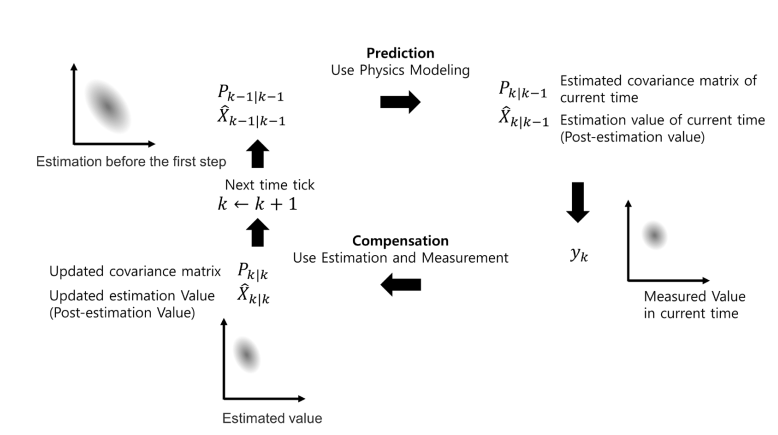
\includegraphics[width=\linewidth]{figures/BasicConceptKalmanFilter.png}
  \caption{Bộ lọc Kalman\cite{pyo2017ros}}
  \label{fig:BasicConceptKalmanFilter}
\end{figure}

\subsubsection*{Particle Filter}
Particle filter là giải thuật phổ biến nhất trong theo dõi vật thể (object tracking). Monte Carlo localization sử dụng bộ lọc Particle. Bộ lọc Kalman chỉ chính xác với hệ tuyến tính và nhiễu theo chuẩn Gaussian. Phần lớn các vấn đề trong thế giới thực là các hệ phi tuyến.

Bởi vì các cảm biến và robot cũng là hệ tuyến tính, bộ lọc particle thường được sử dụng cho ước tính trạng thái vị trí robot. Nếu bộ lọc Kalman tìm kiếm các thông số bằng chuyển động tuyến tính thì bộ lọc Particle filter là một kĩ thuật dự đoán thông qua mô phỏng dựa trên phương pháp thử sai (try-and-error). Bộ lọc này ước tính giá trị bằng phân bố xác suất từng phần trong hệ thống.

Khi sử dụng SLAM, giá trị odometry của robot và các giá trị đo từ cảm biến được sử dụng để ước tính trạng thái hiện tại của robot. Trong phương pháp này, trạng thái vị trí không chắc chắn của robot được mô tả bằng một chùm điểm gọi là các mẫu. Chúng ta di chuyển các điểm tới một vị trí và hướng mới được ước tính dựa trên mô hình chuyển động của robot và xác suất, phép đo trọng số của từng điểm dựa vào giá trị đo thực tế, và giảm nhiễu để ước tính trạng thái chính xác. Trong robot di động, mỗi điểm được biểu diễn bởi trạng thái vị trí (x, y, i), trọng số.

Bộ lọc particle filter gồm 5 bước chính, ngoại trừ bước khởi tạo, các bước còn lại được lặp đi lặp lại để thực hiện ước tính vị trí robot. Nói cách khác, đây là phương pháp ước tính trạng thái vị trí của robot bằng cách cập nhật phân bố của các điểm thông qua xác suất của robot trong hệ tọa độ X, Y dựa trên các giá trị cảm biến đo được.

(1) \textbf{Khởi tạo}:
Vì trạng thái khởi tạo của robot (vị trí và hướng) chưa biết, các điểm dự đoán được phân bố ngẫu nhiên trong phạm vi có thể, với N điểm. Mỗi điểm khởi tạo có trọng số 1/N, và tổng các trọng số của các điểm dự đoán là 1. N được đặt theo kinh nghiệm, thông thường là vài trăm. Nếu vị trí khởi tạo đã biết, các điểm dự đoán được đặt gần với robot.

(2) \textbf{Dự đoán}: Dựa trên mô hình mô tả hệ thống chuyển động của robot, nó dịch chuyển mỗi điểm particle theo giá trị đo từ thông tin odometry và nhiễu.

(3) \textbf{Cập nhật}: Dựa trên thông tin đo được từ các cảm biến, xác suất của mỗi điểm dự đoán được tính toán và giá trị trọng số được cập nhật dựa trên xác suất tính được.

(4) \textbf{Ước tính trạng thái}: Vị trí, hướng và trọng số của tất cả các điểm dự đoán được dùng để tính toán trọng số trung bình, giá trị trung bình và giá trị trọng số lớn nhất cho việc dự đoán trạng thái của robot.

(5) \textbf{Lấy mẫu lại}: Bước này tạo ra các điểm dự đoán mới để loại bỏ các điểm có trọng số thấp và tạo các điểm mới kế thừa từ các điểm được giữ lại, tổng số điểm N phải được duy trì.

\subsection{Định vị và tạo bản đồ đồng thời - SLAM}}

SLAM - Simultaneous Localization And Mapping. Đây là một trong các vấn đề khó nhất của robotics. Vấn đề SLAM nảy sinh khi robot không có bản đồ của môi trường và cũng không biết trạng thái vị trí của chính nó. Thay vào đó là dữ liệu đo ${z}_{1:t}$ và tín hiệu điều khiển ${u}_{1:t}$. Thuật ngữ SLAM mô tả kết quả của vấn đề: Trong SLAM, robot đạt được một bản đồ môi trường trong khi đồng thời định vị nó ở đâu trong bản đồ đó. Bài toán SLAM khó hơn bài toán định vị bởi vì bản đồ chưa biết trước và nó phải được ước tính vị trí theo một quãng đường dài. Nõ cũng khó hơn bài toán tạo bản đồ vì trạng thái vị trí robot chưa biết và nó cũng phải được ước tính trong quãng đường dài.

Như một bài toán con gà và quả trứng, bởi vì trong robot di động muốn định vị tốt thì cần phải có bản đồ chính xác và muốn tạo được bản đồ chính xác thì lại phải định vị tốt.

Theo luật xác suất, có hai dạng chính của SLAM, cả hai dạng này đều quan trọng như nhau. Một dạng là SLAM online. Nó thực hiện các dự đoán qua các trạng thái hiện tại xuyên suốt bản đồ:

\begin{equation}
  p\left({x}_{t}, m | {z}_{1:t}, {u}_{1:t}\right)
\end{equation}

Trong đó, ${x}_{t}$ là trạng thái vị trí tại thời điểm $t$, $m$ là bản đồ, và ${z}_{1:t}$ và ${u}_{1:t}$ là các giá trị đo và điều khiển tương ứng. Vấn đề này gọi là SLAM online vì nó chỉ dự đoán các biến tại thời điểm $t$k, bỏ qua các dữ liệu đo và điều khiển cũ một khi các dữ liệu đó đã được xử lý. Mô hình online SLAM được thể hiện như trong \figurename{ \ref{fig:onlineSLAM}

\begin{figure}[htbp]
  \centering
  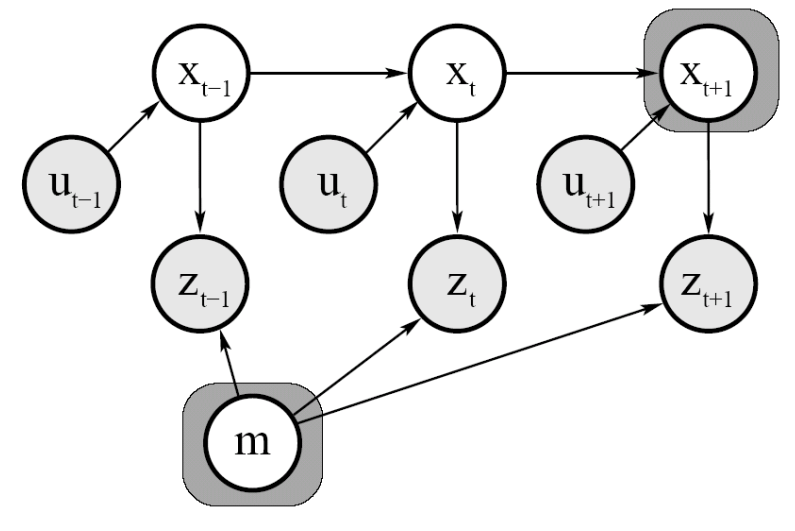
\includegraphics[width=0.6\linewidth]{figures/onlineSLAM.PNG}
  \caption{Online SLAM}
  \label{fig:onlineSLAM}
\end{figure}

Vấn đề SLAM thứ hai là được gọi là \textit{full SLAM}. Trong full SLAM, chúng ta tính toán toàn bộ đường đi ${x}_{1:t}$ xuyên suốt bản đồ, thay vì chỉ trạng thái hiện tại ${x}_{t}$
\begin{equation}
  p\left({x}_{1:t},m | {z}_{1:t}, {u}_{1:t}\right)
\end{equation}

\begin{figure}[htbp]
  \centering
  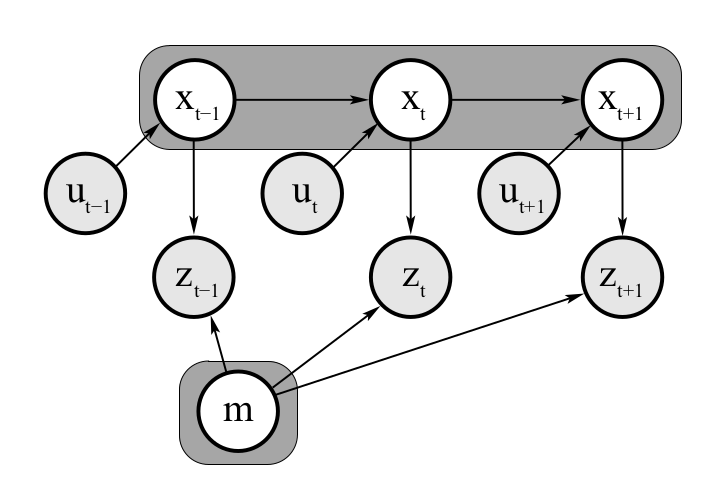
\includegraphics[width=0.6\linewidth]{figures/fullSLAM.png}
  \caption{Full SLAM}
  \label{fig:fullSLAM}
\end{figure}

Sự khác nhau giữa online và full SLAM tạo nên sự phân nhánh trong các thuật toán tương ứng với mỗi loại. Cụ thể, online SLAM là kết quả của việc tích hợp trạng thái robot cũ từ full SLAM.

Một đặc điểm quan trọng nữa của SLAM đó là nó có hai thành phần liên tục và rời rạc. Vấn đề liên tục là ước tính vị trí của các vật thể, đối tượng trong bản đồ và các biến số đặt ra của robot. Các đối tượng có thể là các điểm mốc. Bản chất rời rạc liên quan đến sự tương ứng của các vật thể nó phát hiện được, nó phải xem xét vật thể đó đã được phát hiện ở bước trước đó hay chưa.

% \section{Một số bài toán thực tế trong điều hướng robot}






%% ===================
%%% Local Variables:
%%% mode: latex
%%% TeX-master: "../LuanVanThS_v1.0_main"
%%% End:
